\chapter{Current results Year2}
\label{a:appendix}

From last year the software has been completed and can handle neutrino and muon beam events in a generic MIND type detector. The main problem used to be how to handle multiple hit occupancy but this changed to be an issue with momentum reconstruction. The problem arose from bugs and incorrect use of the third-party software RecPack which is a kalman filter fitter. There are still some issues with the pull plots however it has been improved considerately and the bugs are understood. The main issue seems to be an underestimation of the error for low momentum values. See figures~\ref{fig:mommu}, ~\ref{fig:momantimu}, ~\ref{fig:meanmu}, ~\ref{fig:meanantimu}, ~\ref{fig:sigmamu}, ~\ref{fig:sigmaantimu}.

Figure~\ref{fig:fullrec} shows the current reconstruction efficiency, using simulated data in Baby MIND, defined as the number of reconstructed tracks from the number of identified trajectories and reconstructed with a momentum non-zero to remove errors in the code. For a single muon beam, the efficiency is more than 95\% for the expected full range (0.2-10 GeV/c). Figure~\ref{fig:fullcharge} shows the current charge identification efficiency, which is defined as the number of tracks with the correctly assigned charge out of all the reconstructed trajectories.  For a single muon beam, the efficiency is more than 95\% above 0.8 GeV/c and above 80\% in the region 0.2-0.8GeV/c.

\begin{figure}[h!]
	\begin{minipage}{0.49\linewidth}
		\centerline{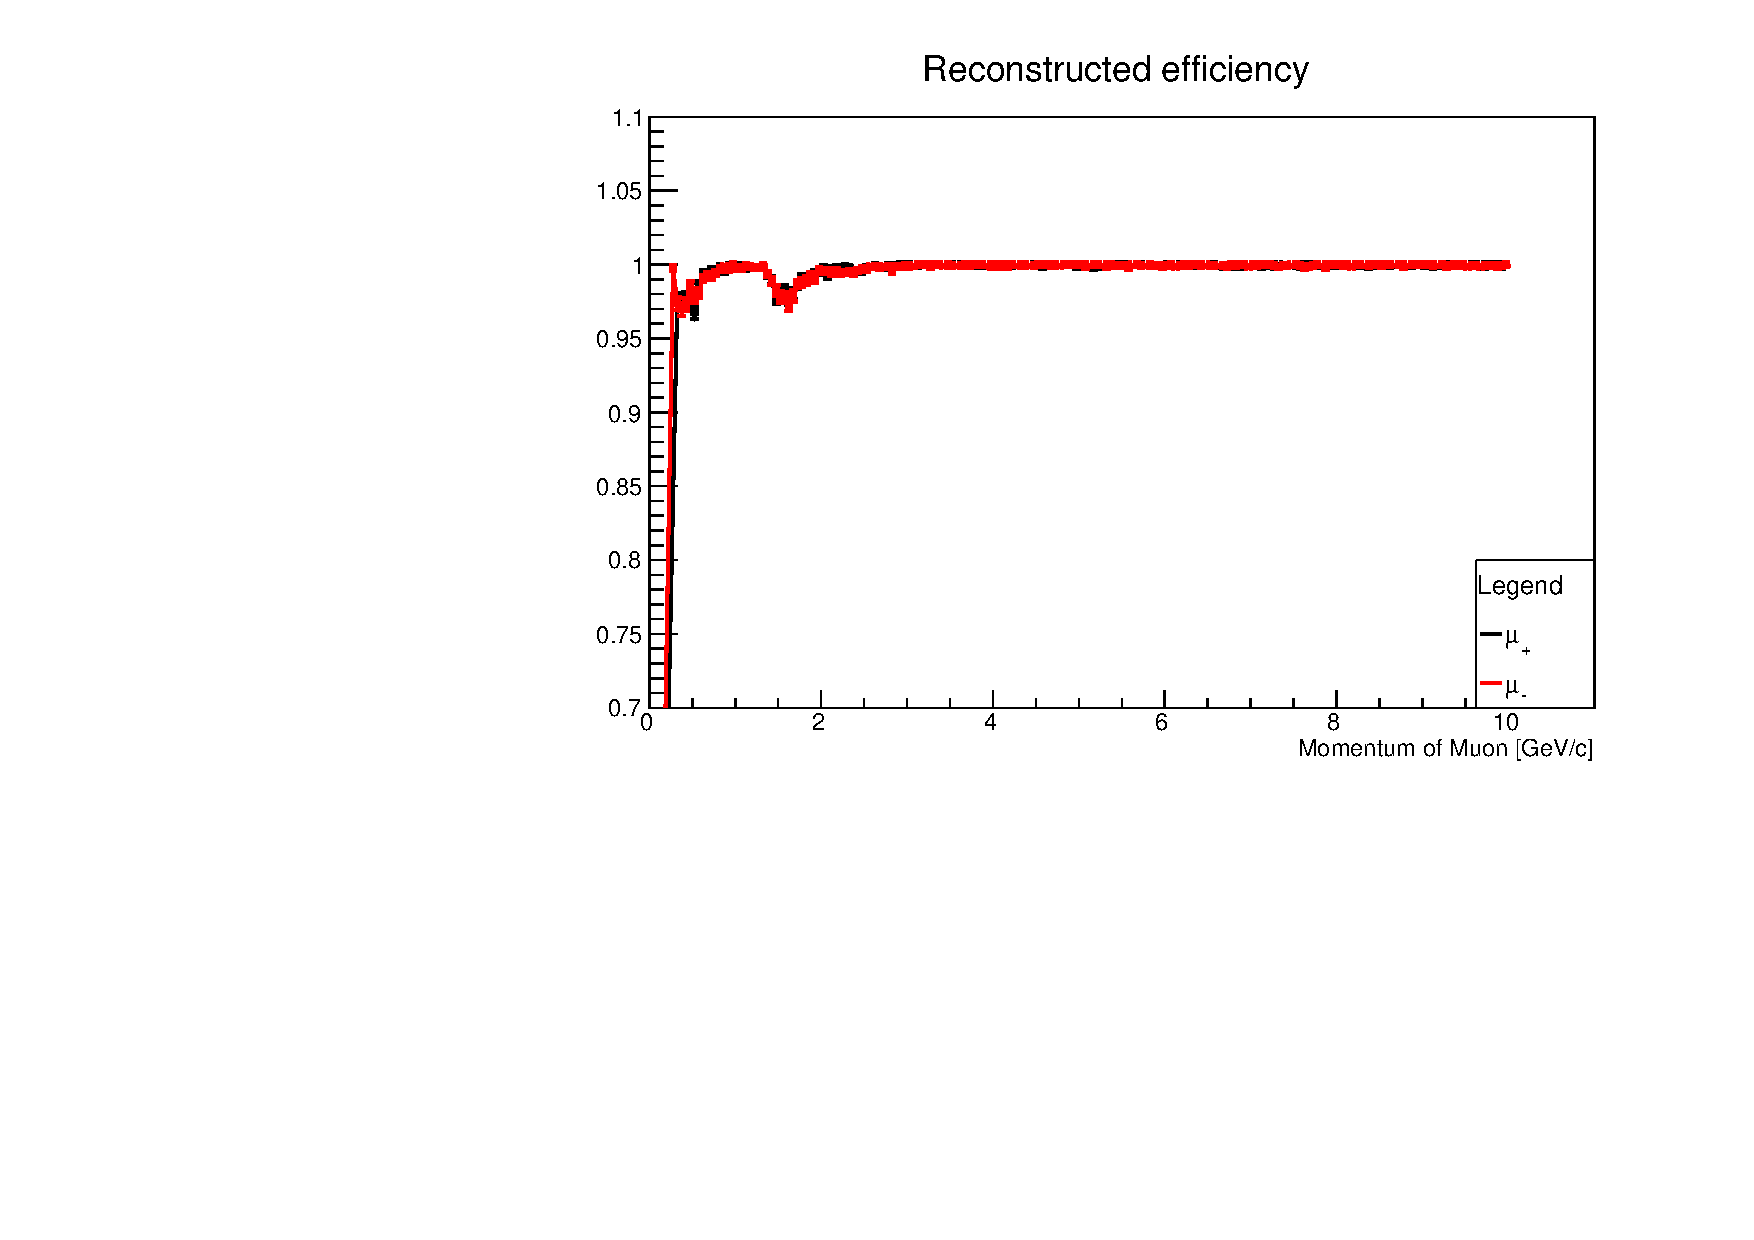
\includegraphics[width=0.9\linewidth]{figures/FullFitted.pdf}}
		%\caption[]{ Reconstruction efficiency: out of identified trajectories, how many are reconstructed?}
			\caption[]{Reconstruction efficiency for a single muon beam}
		\label{fig:fullcharge}
	\end{minipage}
	\hfill
	\begin{minipage}{0.49\linewidth}
		\centerline{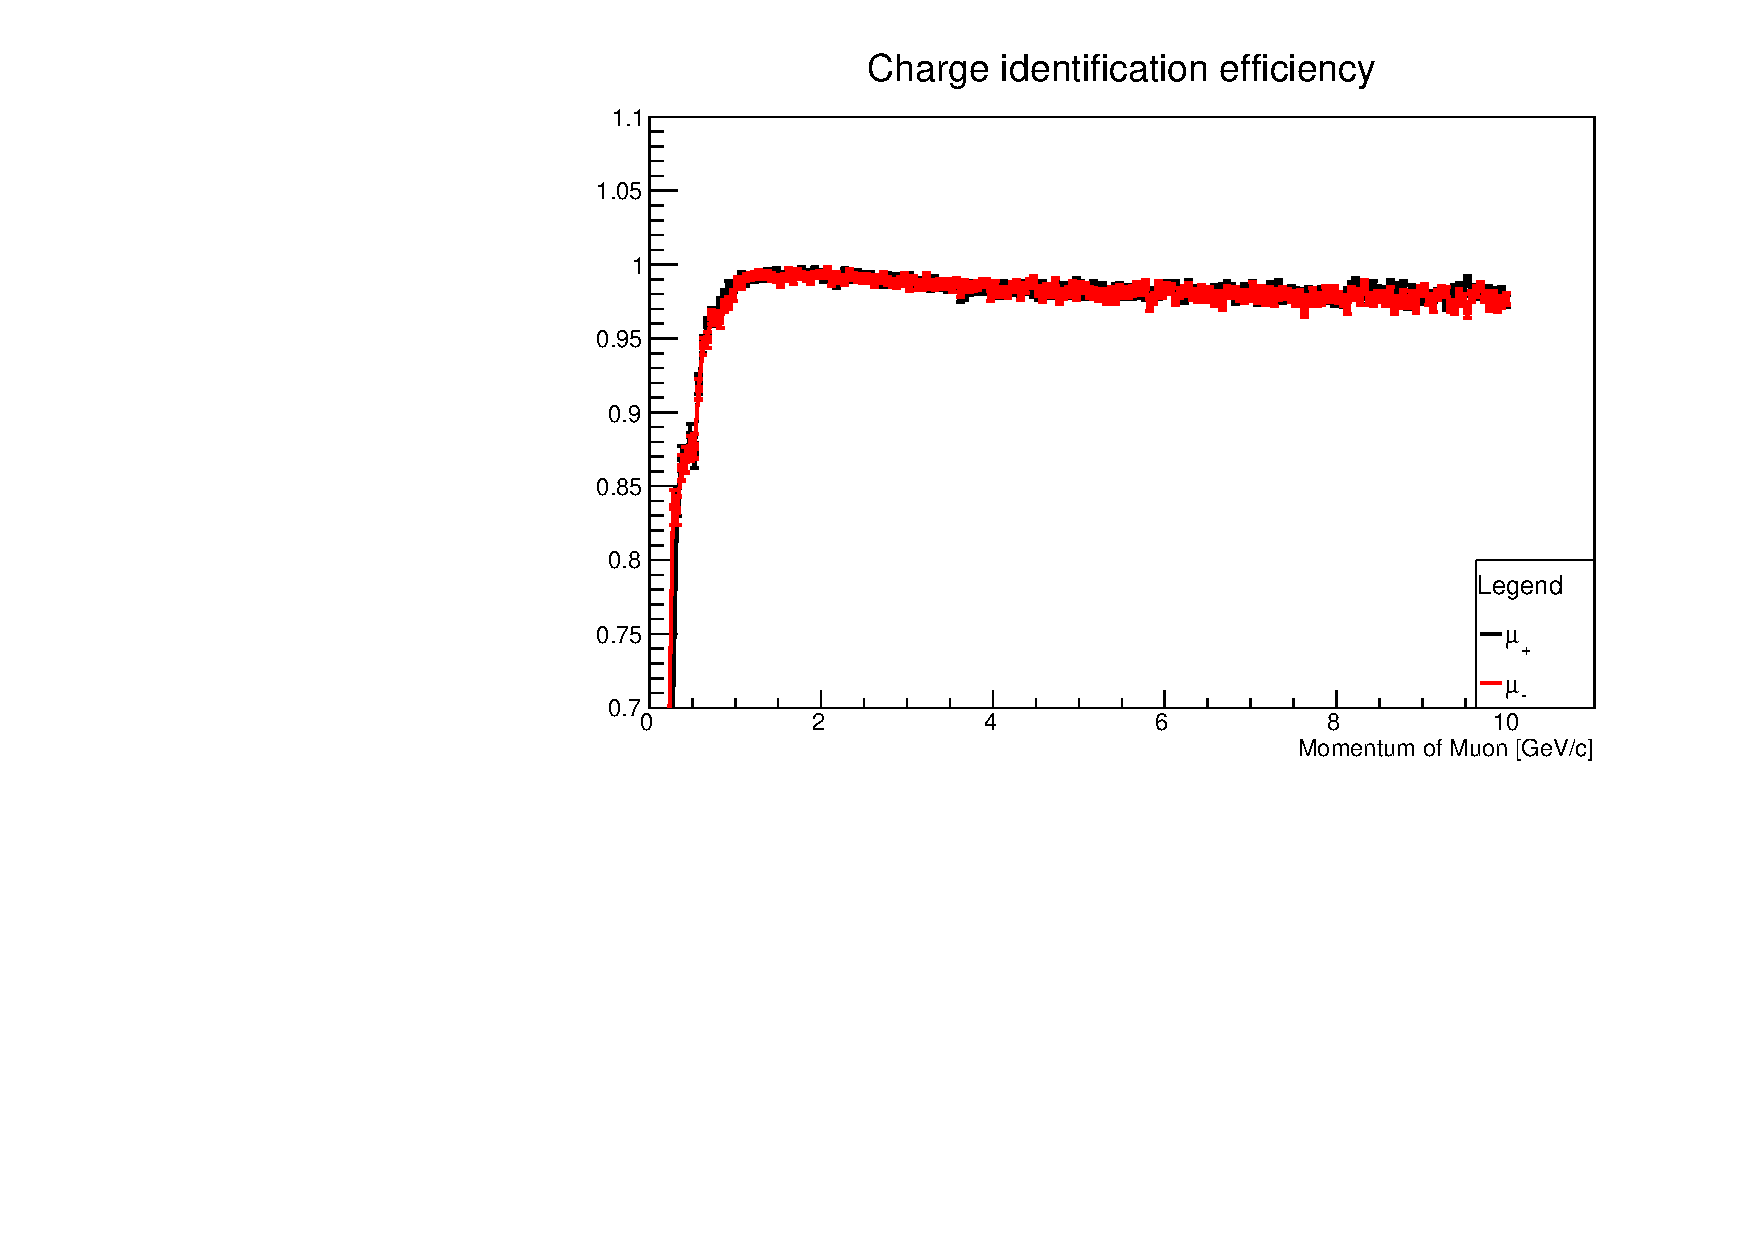
\includegraphics[width=0.9\textwidth]{figures/FullChargeID.pdf}}
		\caption[]{Charge identification efficiency for a single muon beam}
		%	\caption[]{Charge identification efficiency: out of reconstructed trajectories, how many are identified with the correct charge?
		\label{fig:fullrec}
	\end{minipage}
\end{figure}


\begin{figure}[h!]
	\begin{minipage}{0.49\linewidth}
		\centerline{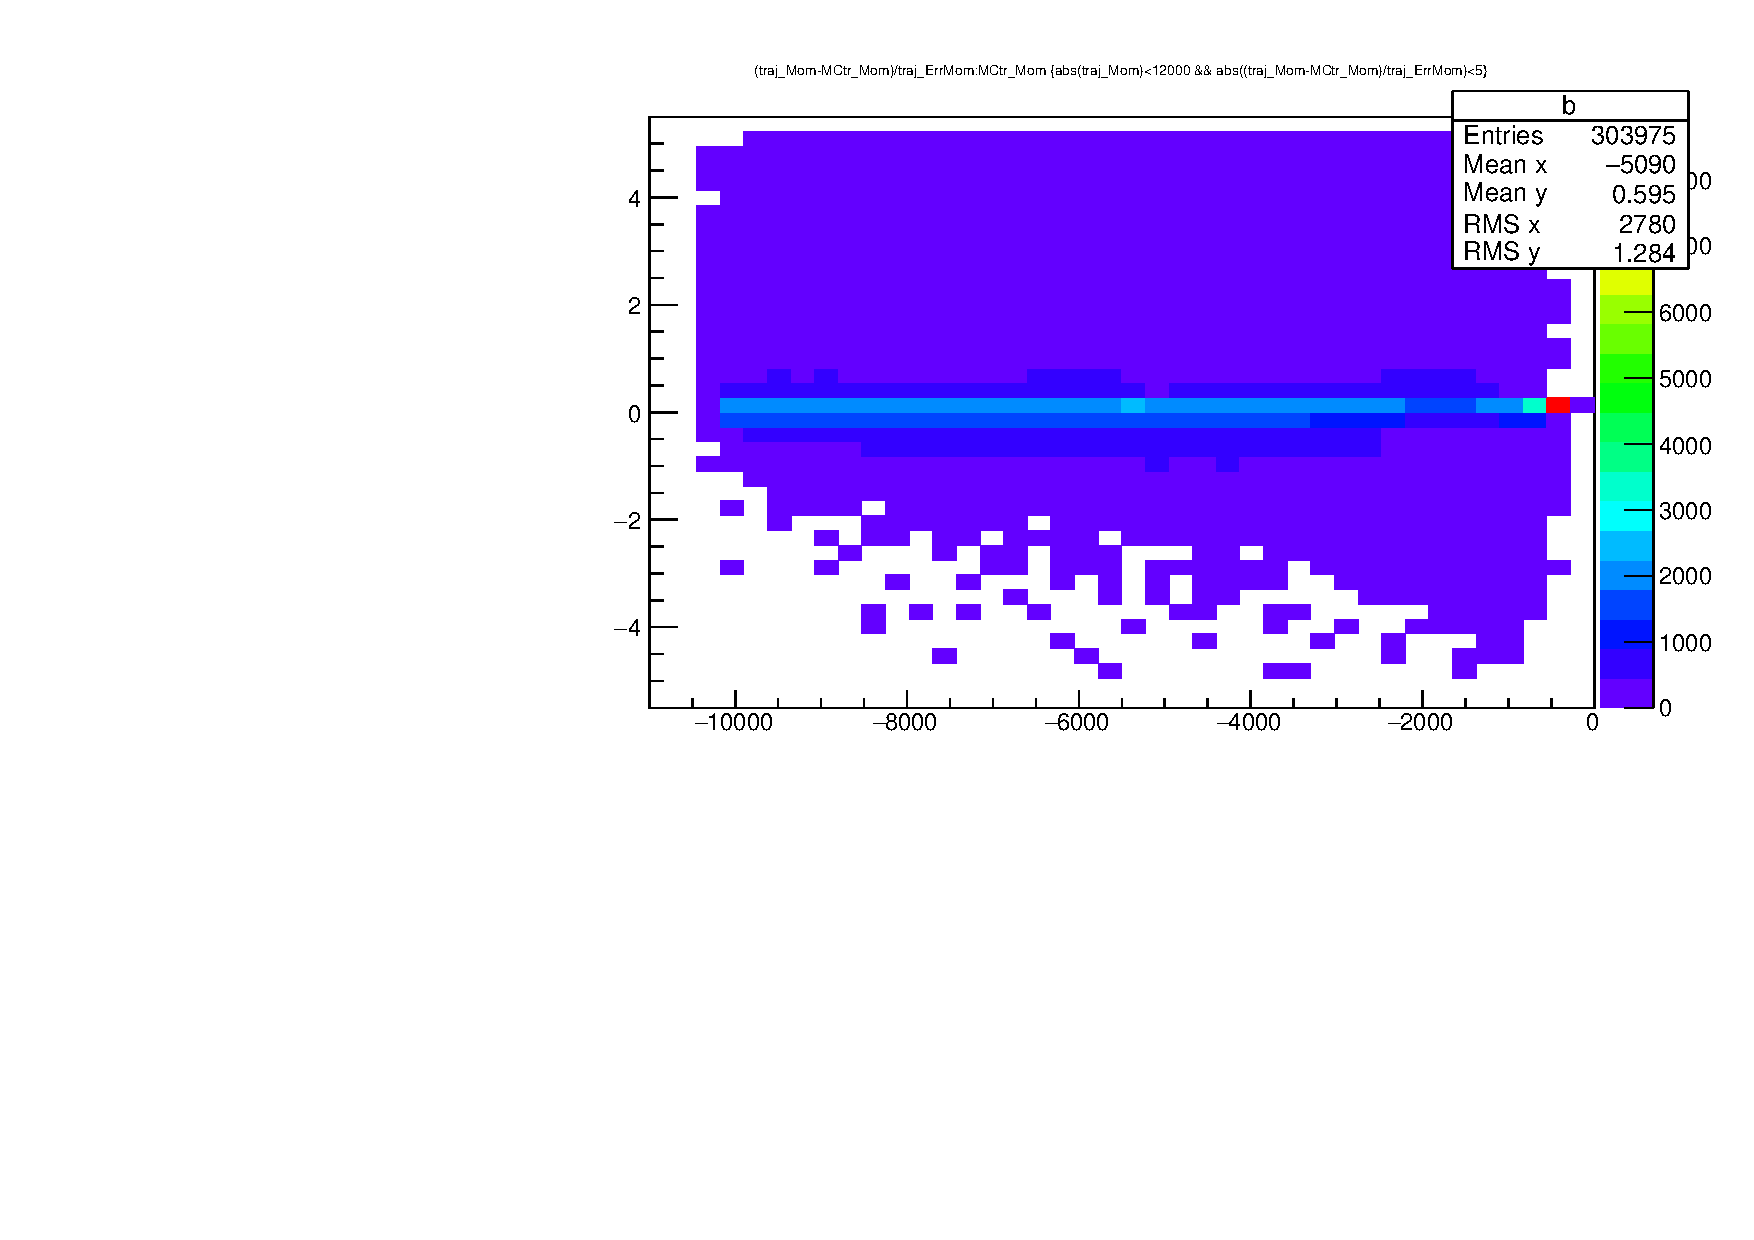
\includegraphics[width=0.9\linewidth]{figures/mupull.pdf}}
		%\caption[]{ Reconstruction efficiency: out of identified trajectories, how many are reconstructed?}
			\caption[]{Momentum pull plot for a single $\mu^-$ beam}
		\label{fig:mommu}
	\end{minipage}
	\hfill
	\begin{minipage}{0.49\linewidth}
		\centerline{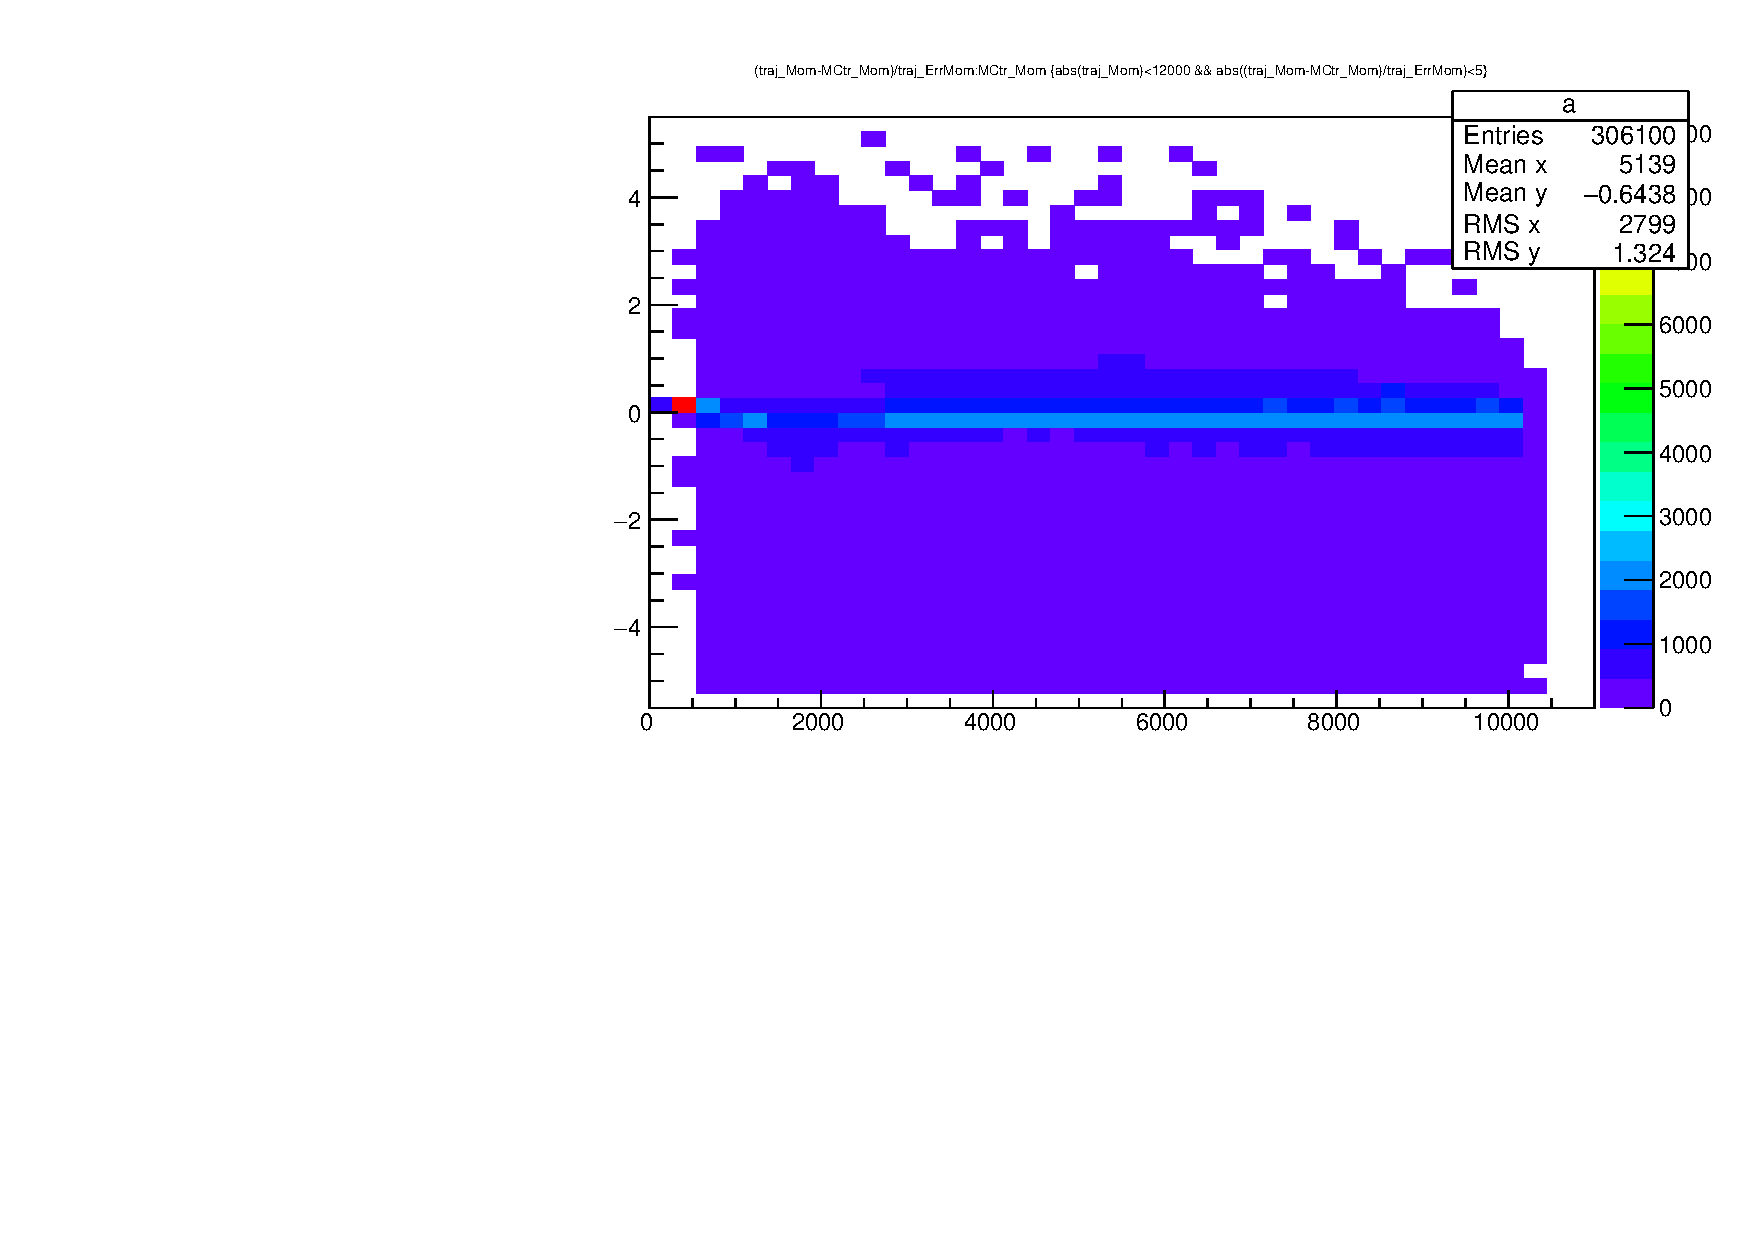
\includegraphics[width=0.9\textwidth]{figures/antimupull.pdf}}
		\caption[]{Momentum pull plot for a single $\mu^+$ beam}
		%	\caption[]{Charge identification efficiency: out of reconstructed trajectories, how many are identified with the correct charge?
		\label{fig:momantimu}
	\end{minipage}
\end{figure}

\begin{figure}[h!]
	\begin{minipage}{0.49\linewidth}
		\centerline{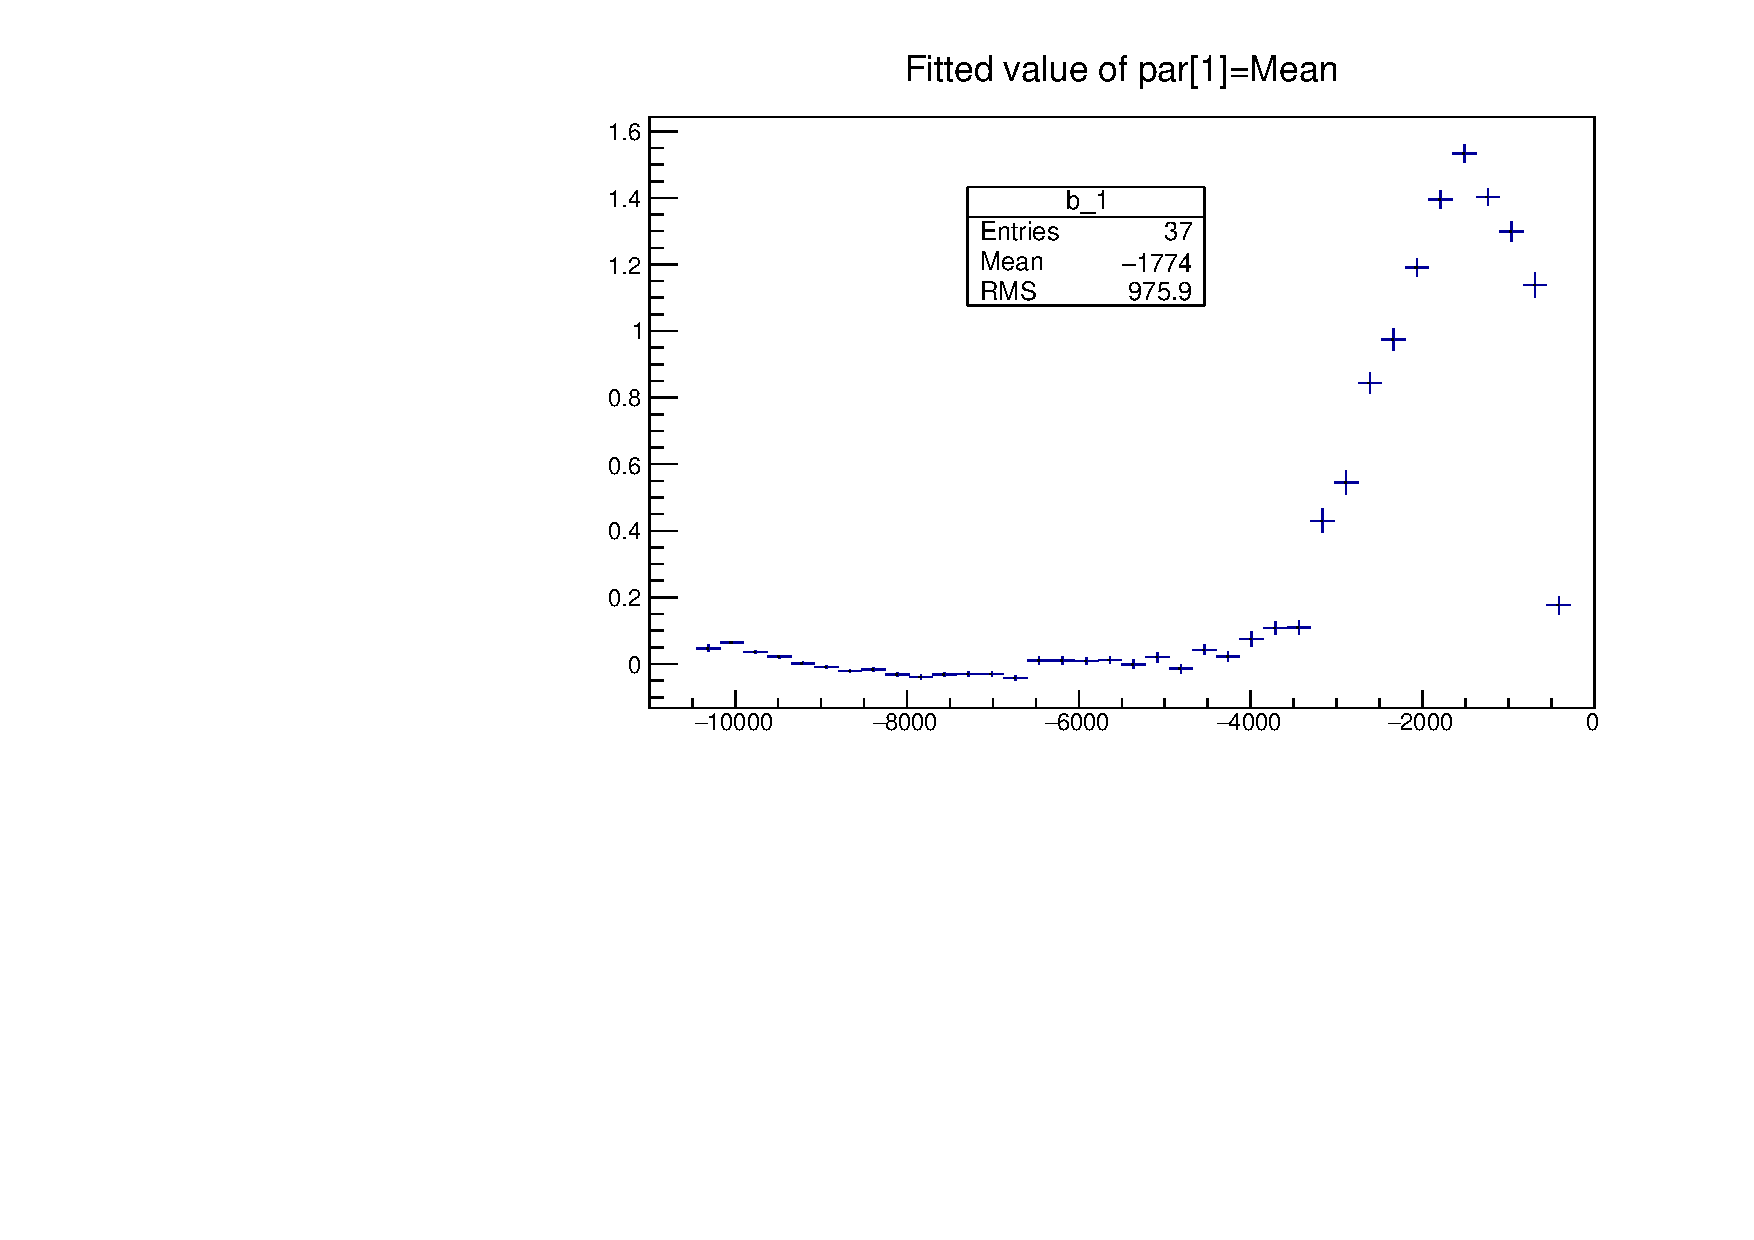
\includegraphics[width=0.9\linewidth]{figures/mumean.pdf}}
		%\caption[]{ Reconstruction efficiency: out of identified trajectories, how many are reconstructed?}
			\caption[]{The mean evolution of the pull plot for a single $\mu^-$ beam}
		\label{fig:meanmu}
	\end{minipage}
	\hfill
	\begin{minipage}{0.49\linewidth}
		\centerline{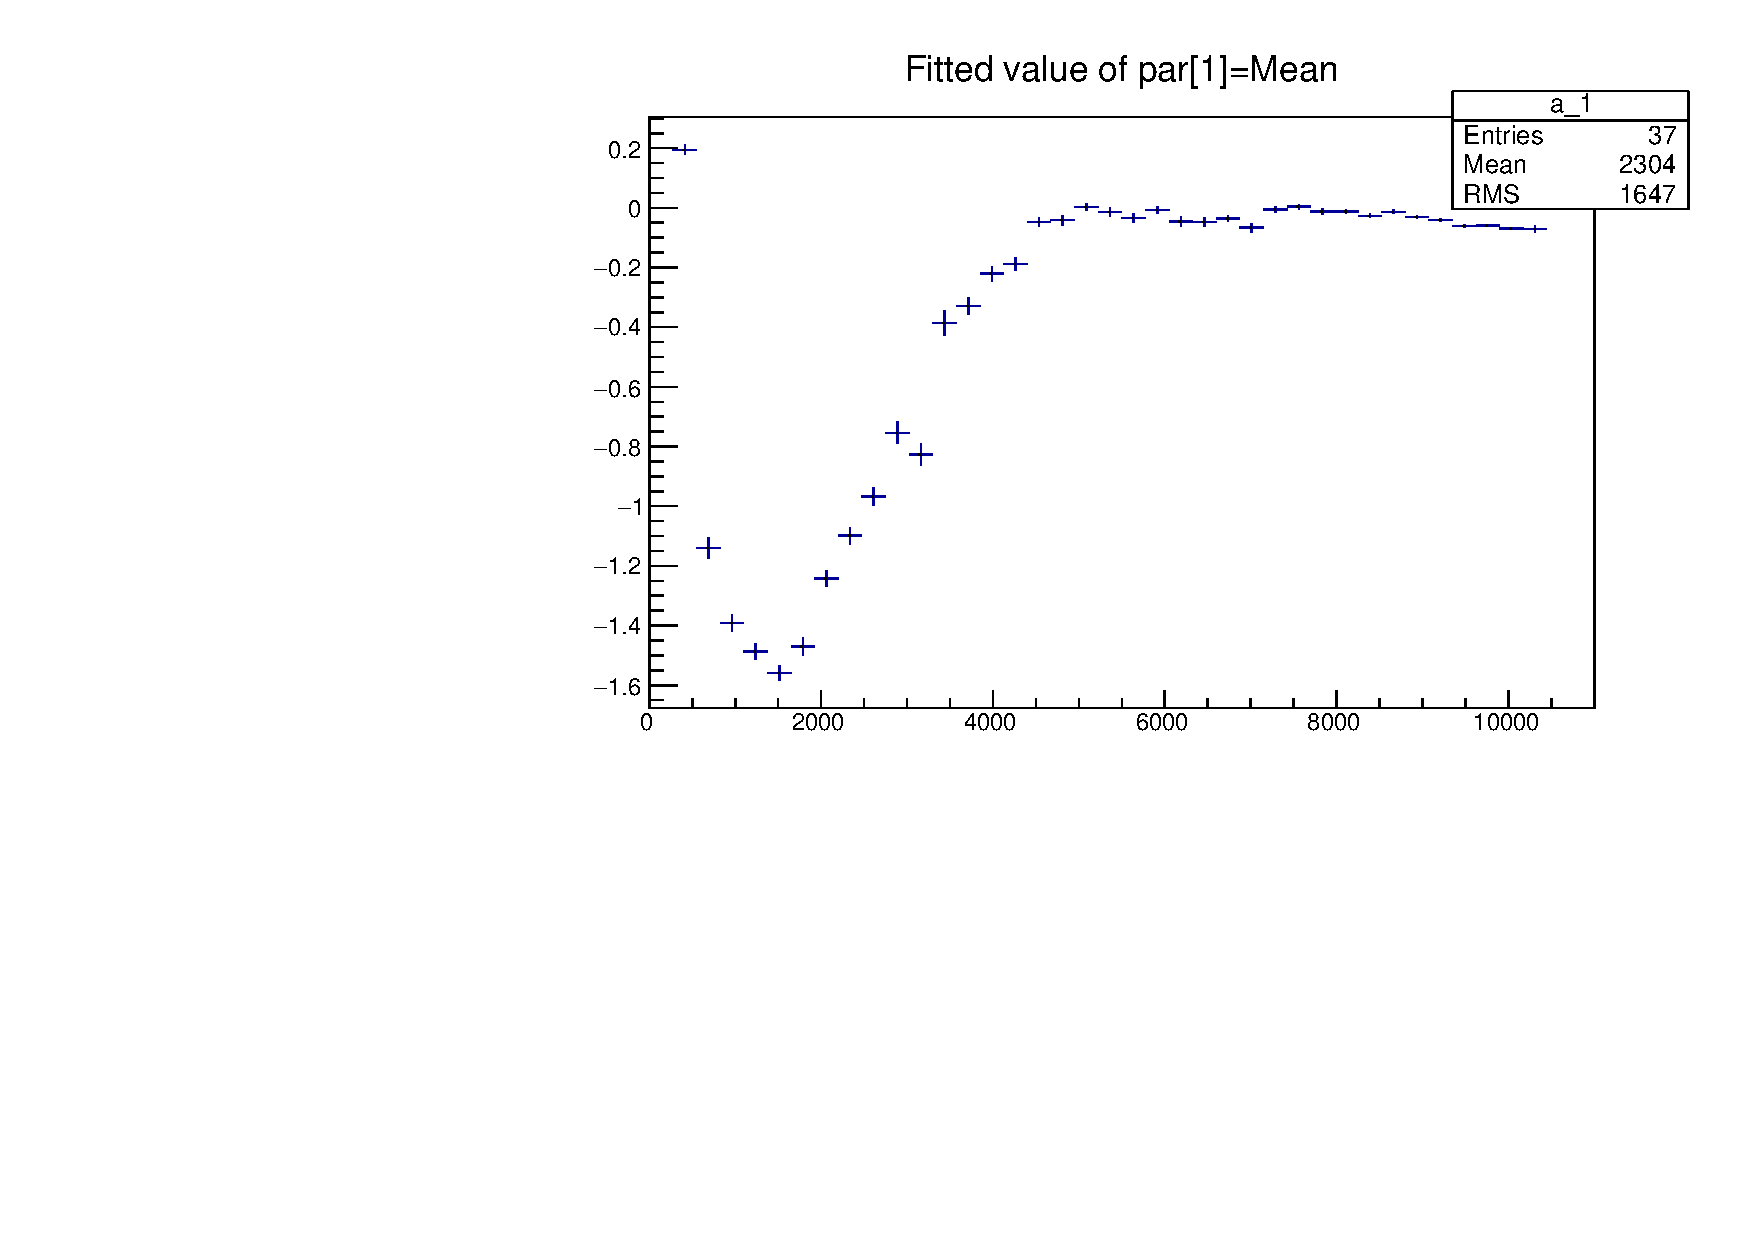
\includegraphics[width=0.9\textwidth]{figures/antimumean.pdf}}
		\caption[]{The mean evolution of the pull plot for a single $\mu^+$ beam}
		%	\caption[]{Charge identification efficiency: out of reconstructed trajectories, how many are identified with the correct charge?
		\label{fig:meanantimu}
	\end{minipage}
\end{figure}

\begin{figure}[h!]
	\begin{minipage}{0.49\linewidth}
		\centerline{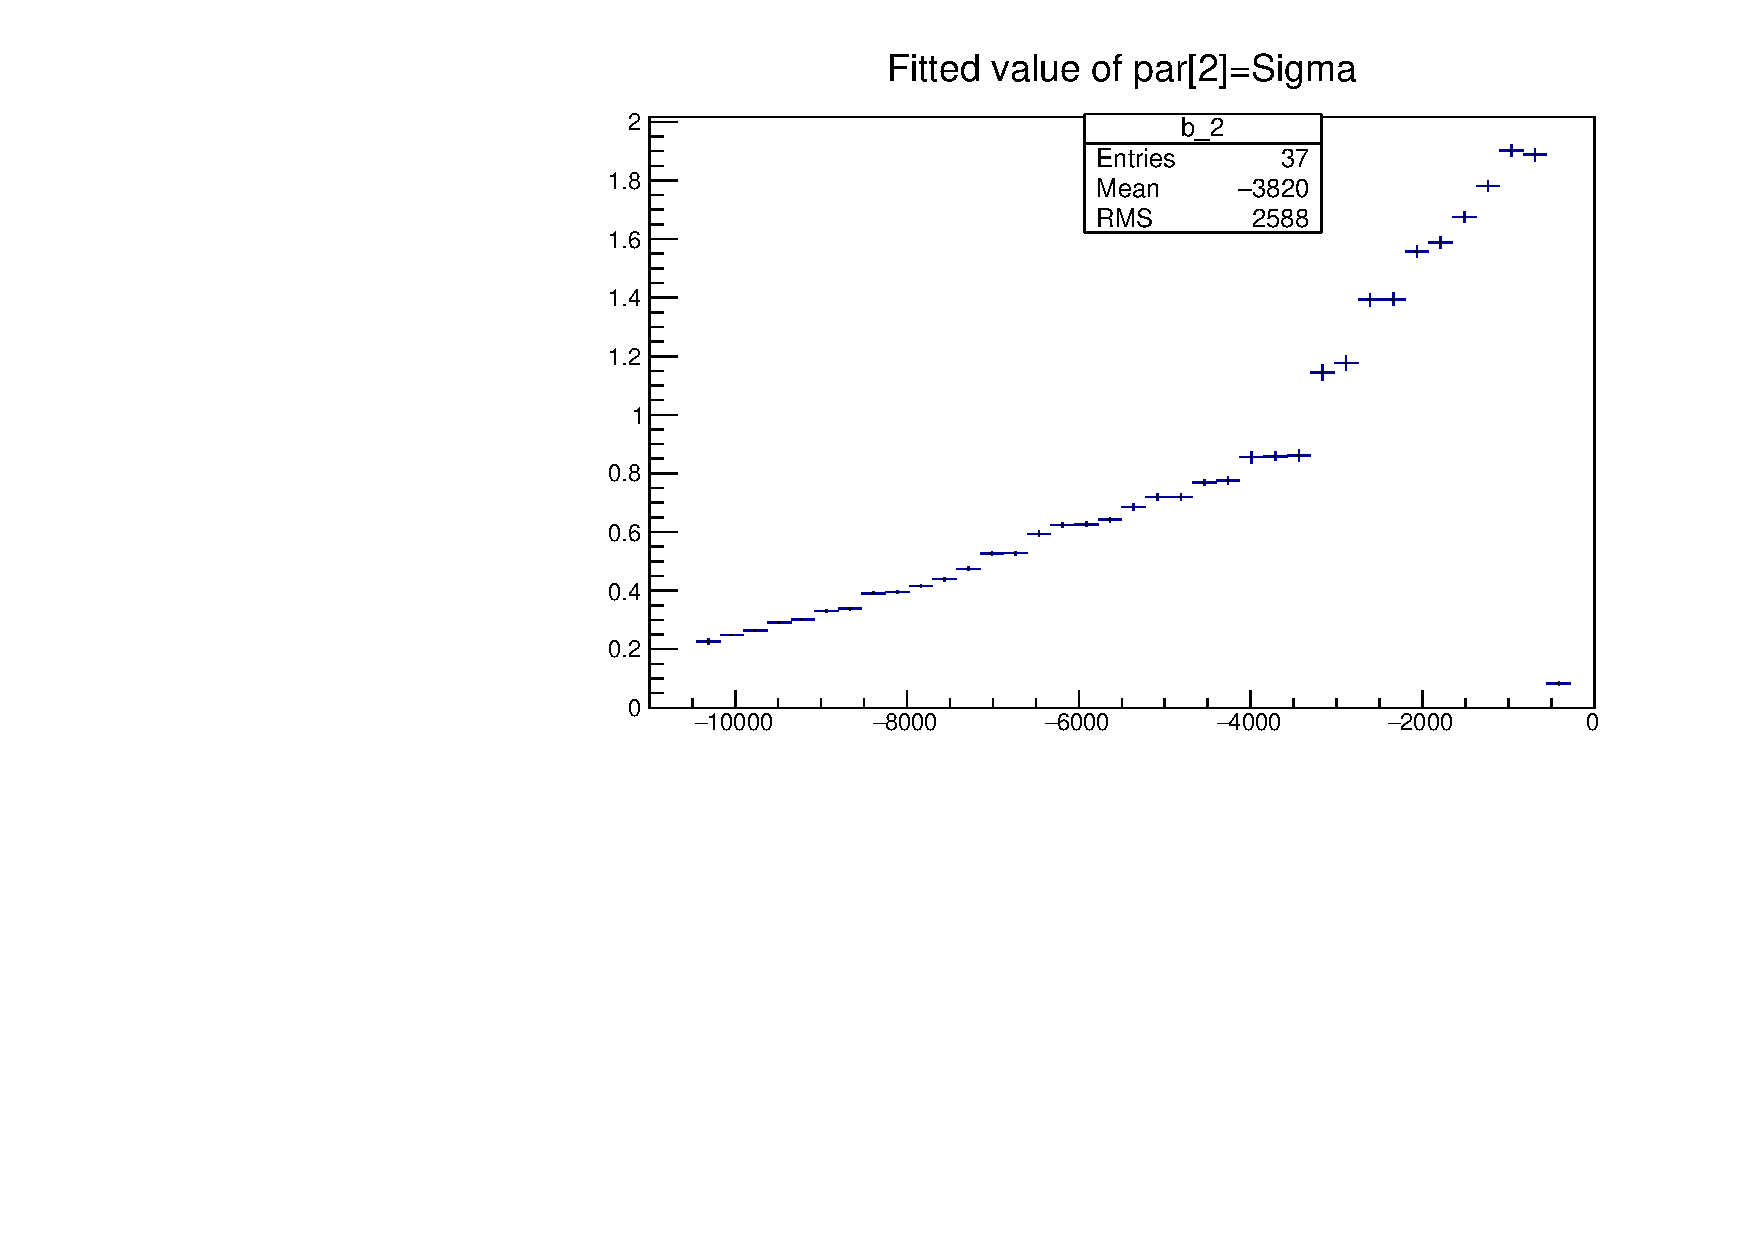
\includegraphics[width=0.9\linewidth]{figures/musigma.pdf}}
		%\caption[]{ Reconstruction efficiency: out of identified trajectories, how many are reconstructed?}
			\caption[]{The sigma evolution of the pull plot for a single $\mu^-$ beam}
		\label{fig:sigmamu}
	\end{minipage}
	\hfill
	\begin{minipage}{0.49\linewidth}
		\centerline{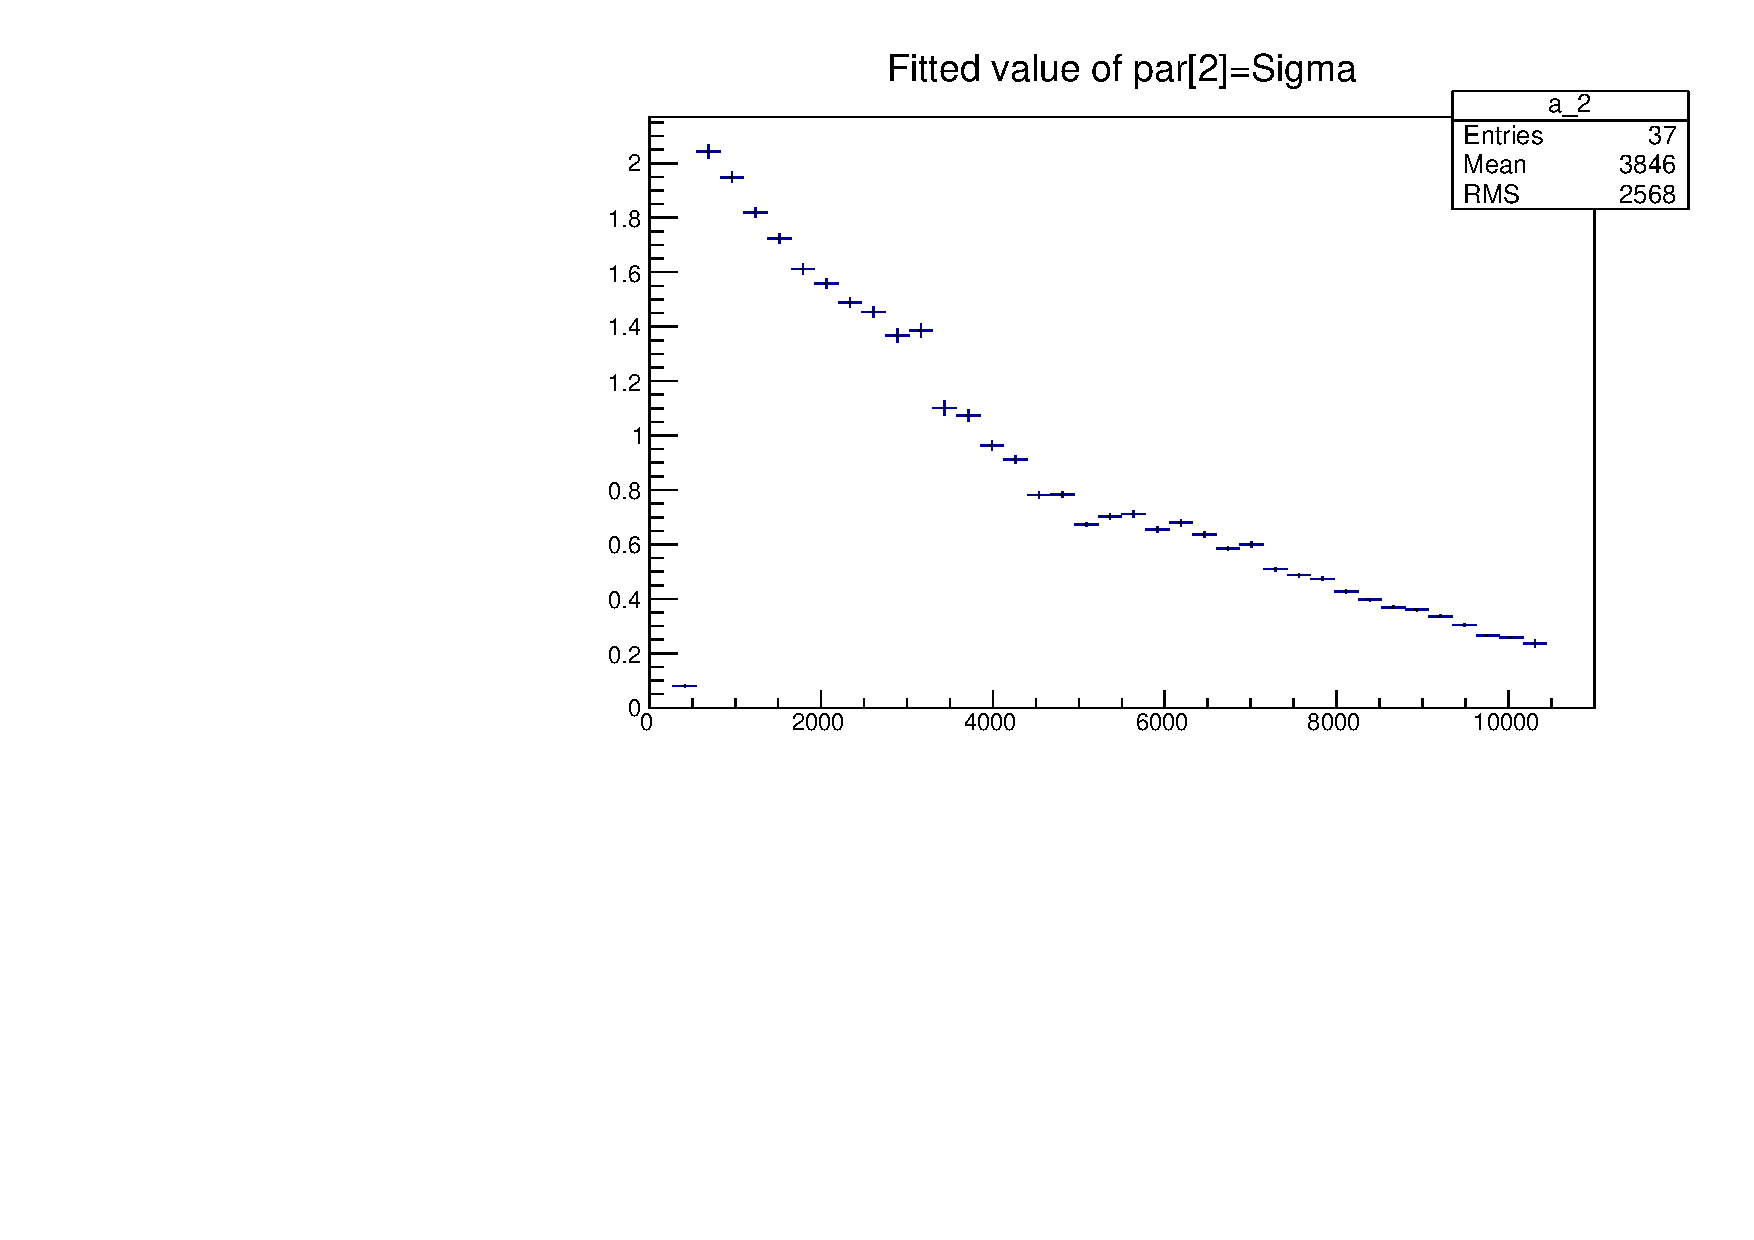
\includegraphics[width=0.9\textwidth]{figures/antimusigma.pdf}}
		\caption[]{The sigma evolution of the pull plot for a single $\mu^+$ beam}
		%	\caption[]{Charge identification efficiency: out of reconstructed trajectories, how many are identified with the correct charge?
		\label{fig:sigmaantimu}
	\end{minipage}
\end{figure}

During June-July 2016 a test beam was performed to characterise the readout system, data acquisition (DAQ) and electronics to be used in the Baby MIND detector. The test beam was at the T9 beam of the East Area, operating at the Proton Synchrotron (PS) at CERN. A Totally Active Scintillation Detector (TASD)~\ref{fig:AIDA} constructed under the AIDA project (Advanced European Infrastructures for Detectors at Accelerators) was used to test the readout system, electronics, DAQ and reconstruction software. For the beam test, twelve planes, consisting of 16 scintillator bars $10\times 10\times 1000$~mm$^3$, read out on both sides by S12571-025C Hamamatsu MPPCs  along alternating $x$ and $y$ directions were instrumented (a total of 384 MPPCs). The beam consisted of muons and pions from $\sim$200~MeV/c up to 10~GeV/c. Figure~\ref{fig:AIDA} shows a schematic of the TASD and figure~\ref{fig:beamProfile} shows the evolution of the beam profile as measured by the TASD during the test beam and reconstructed with the SaRoMan software. 

\begin{figure}[h]
	\begin{minipage}{0.39\linewidth}
		\centerline{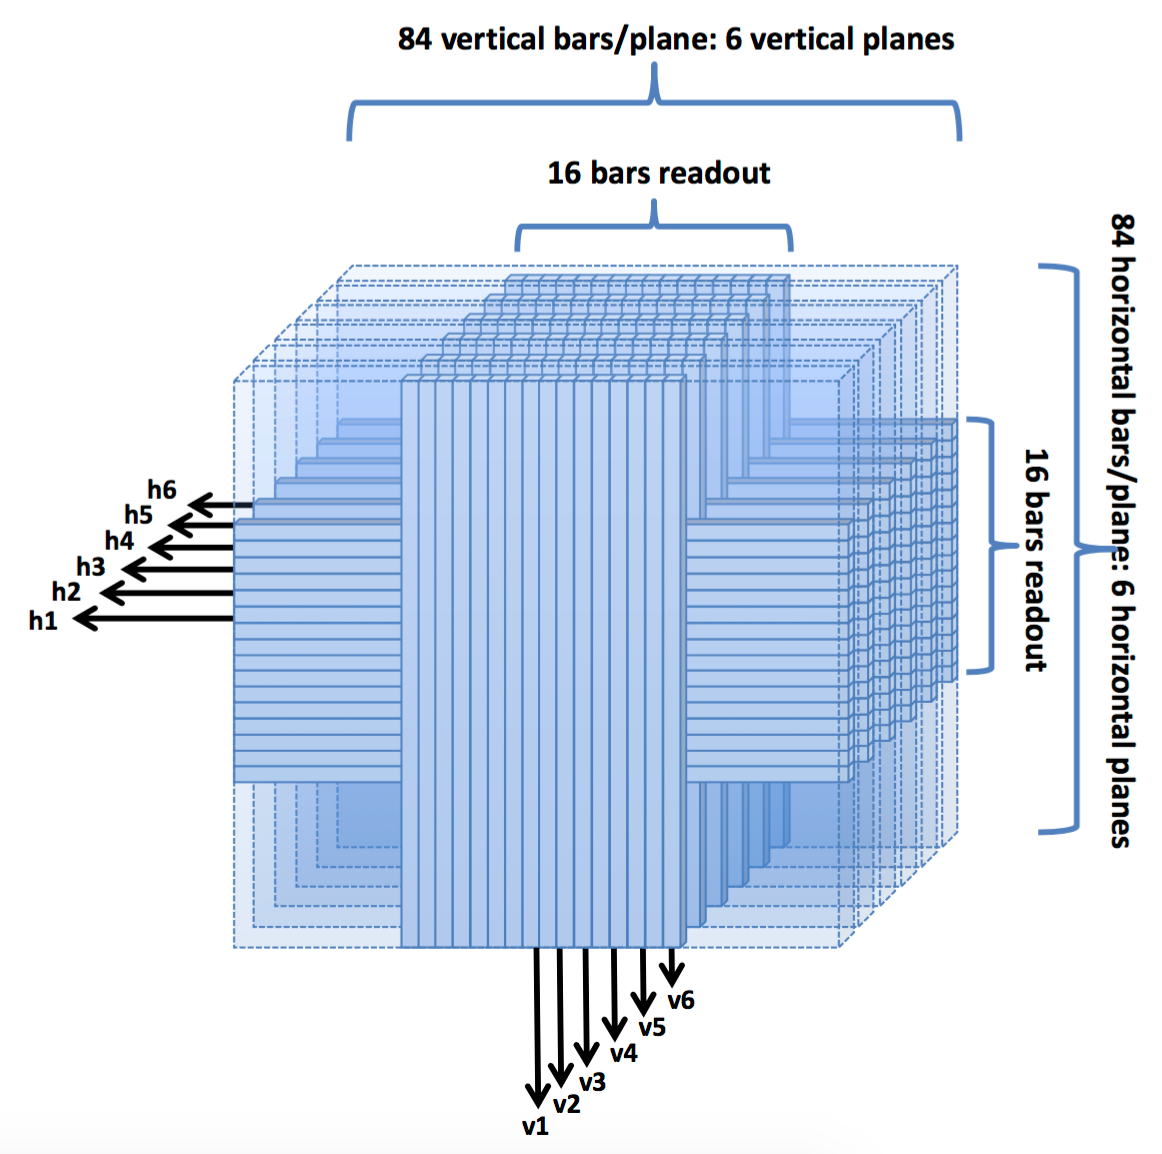
\includegraphics[width=0.9\linewidth]{Figures/AIDA.png}}
		\caption[]{The TASD with the instrumented bars visualised.}
		\label{fig:AIDA}
	\end{minipage}
	\hfill
	\begin{minipage}{0.59\linewidth}
		\centerline{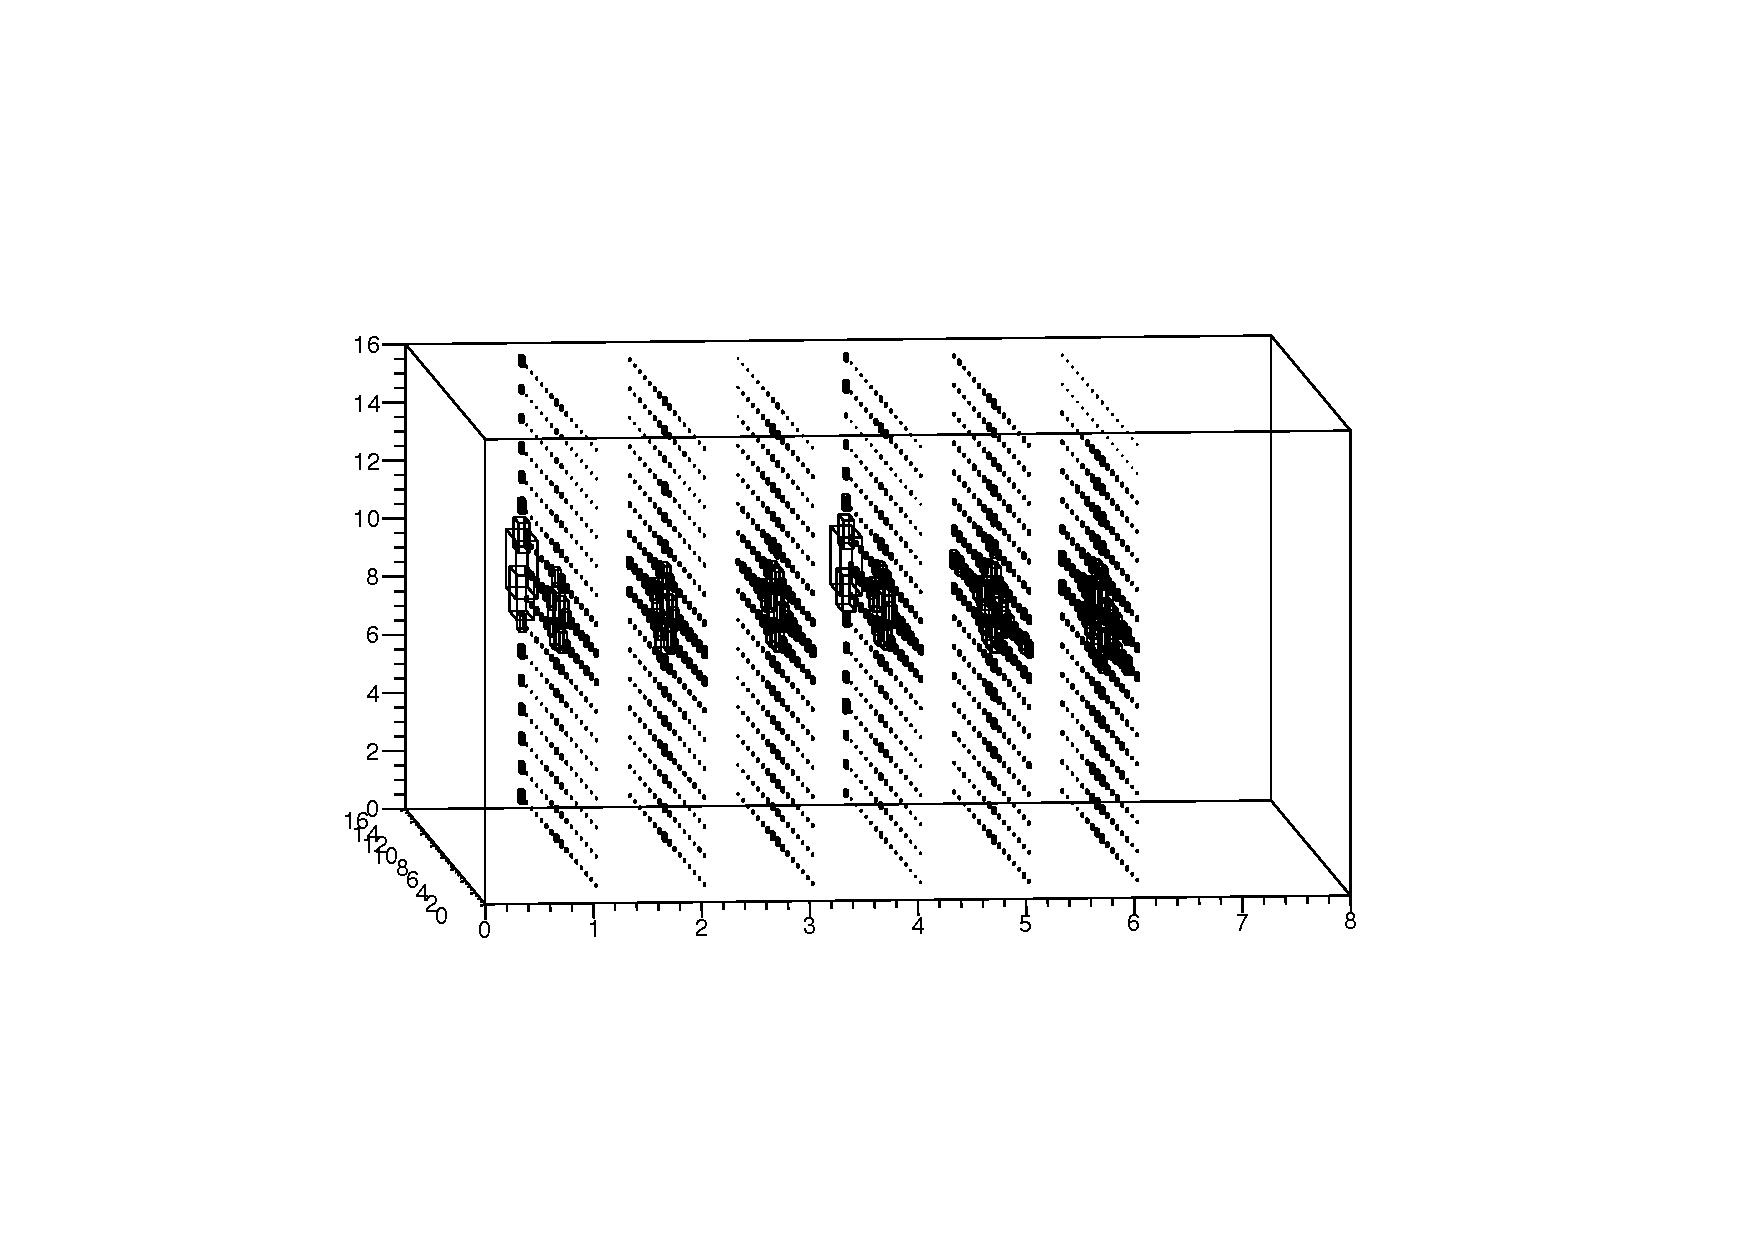
\includegraphics[width=\textwidth, trim = 5cm 5cm 5cm 5cm]{Figures/beamPlot.pdf}}
		\caption[]{Beam profile measured by the TASD.}
		\label{fig:beamProfile}
	\end{minipage}
\end{figure}

Unfortunately for neutrino tracks it would be beneficial to perform simulations with the WAGASCI + Baby MIND but the WAGASCI design has not yet been shared from that collaboration. Instead these neutrino track simulations have been performed using the TASD as a target and then Baby MIND as a muon spectrometer behind it, see~\ref{fig:event} figure~\ref{fig:schematic}. Also for visualization a sample event has been added. The efficiency plots provided,figures~\ref{fig:numufitted} ,~\ref{fig:numucharge},~\ref{fig:antinumufitted} and ~\ref{fig:antinumucharge}, require more data to be fully understood, they do however look promising. Something which needs to be further understood is the pull plots which may indicate an issue for the momentum reconstruction, figures~\ref{fig:numumom}  and ~\ref{fig:antinumumom}, to handle tracks which start off at an angle compared to the beam direction.

\begin{figure}[h!]
	\begin{minipage}{0.49\linewidth}
		\centerline{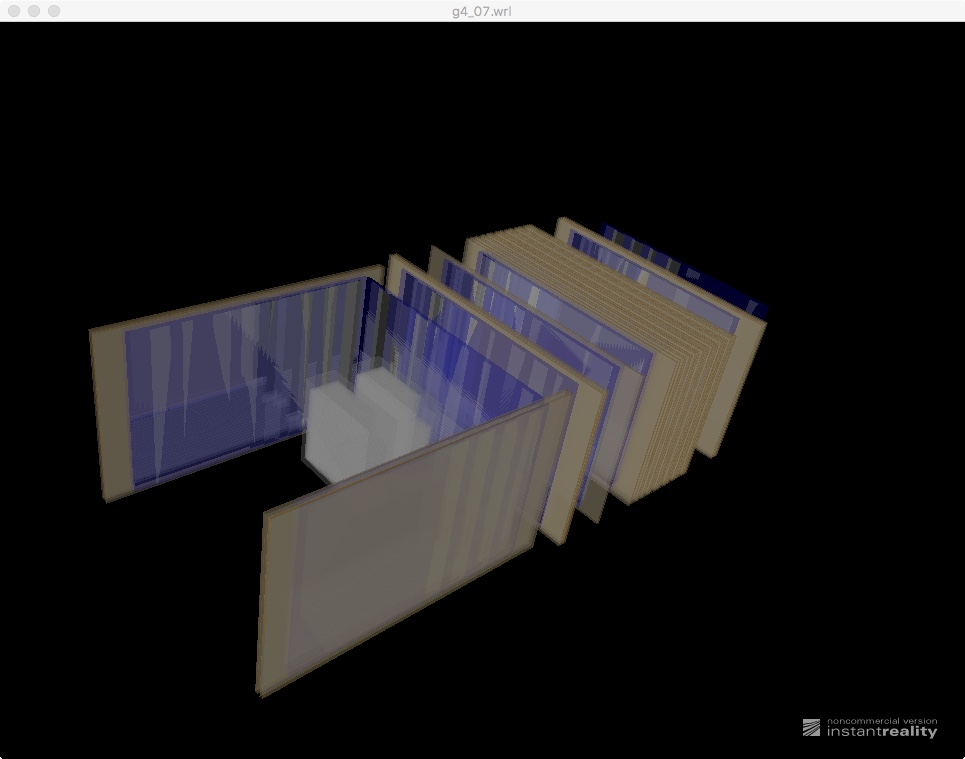
\includegraphics[width=0.9\linewidth]{figures/mindSide.jpeg}}
		%\caption[]{ Reconstruction efficiency: out of identified trajectories, how many are reconstructed?}
			\caption[]{A schematic for the TASD + babyMIND detector}
		\label{fig:schematic}
	\end{minipage}
	\hfill
	\begin{minipage}{0.49\linewidth}
		\centerline{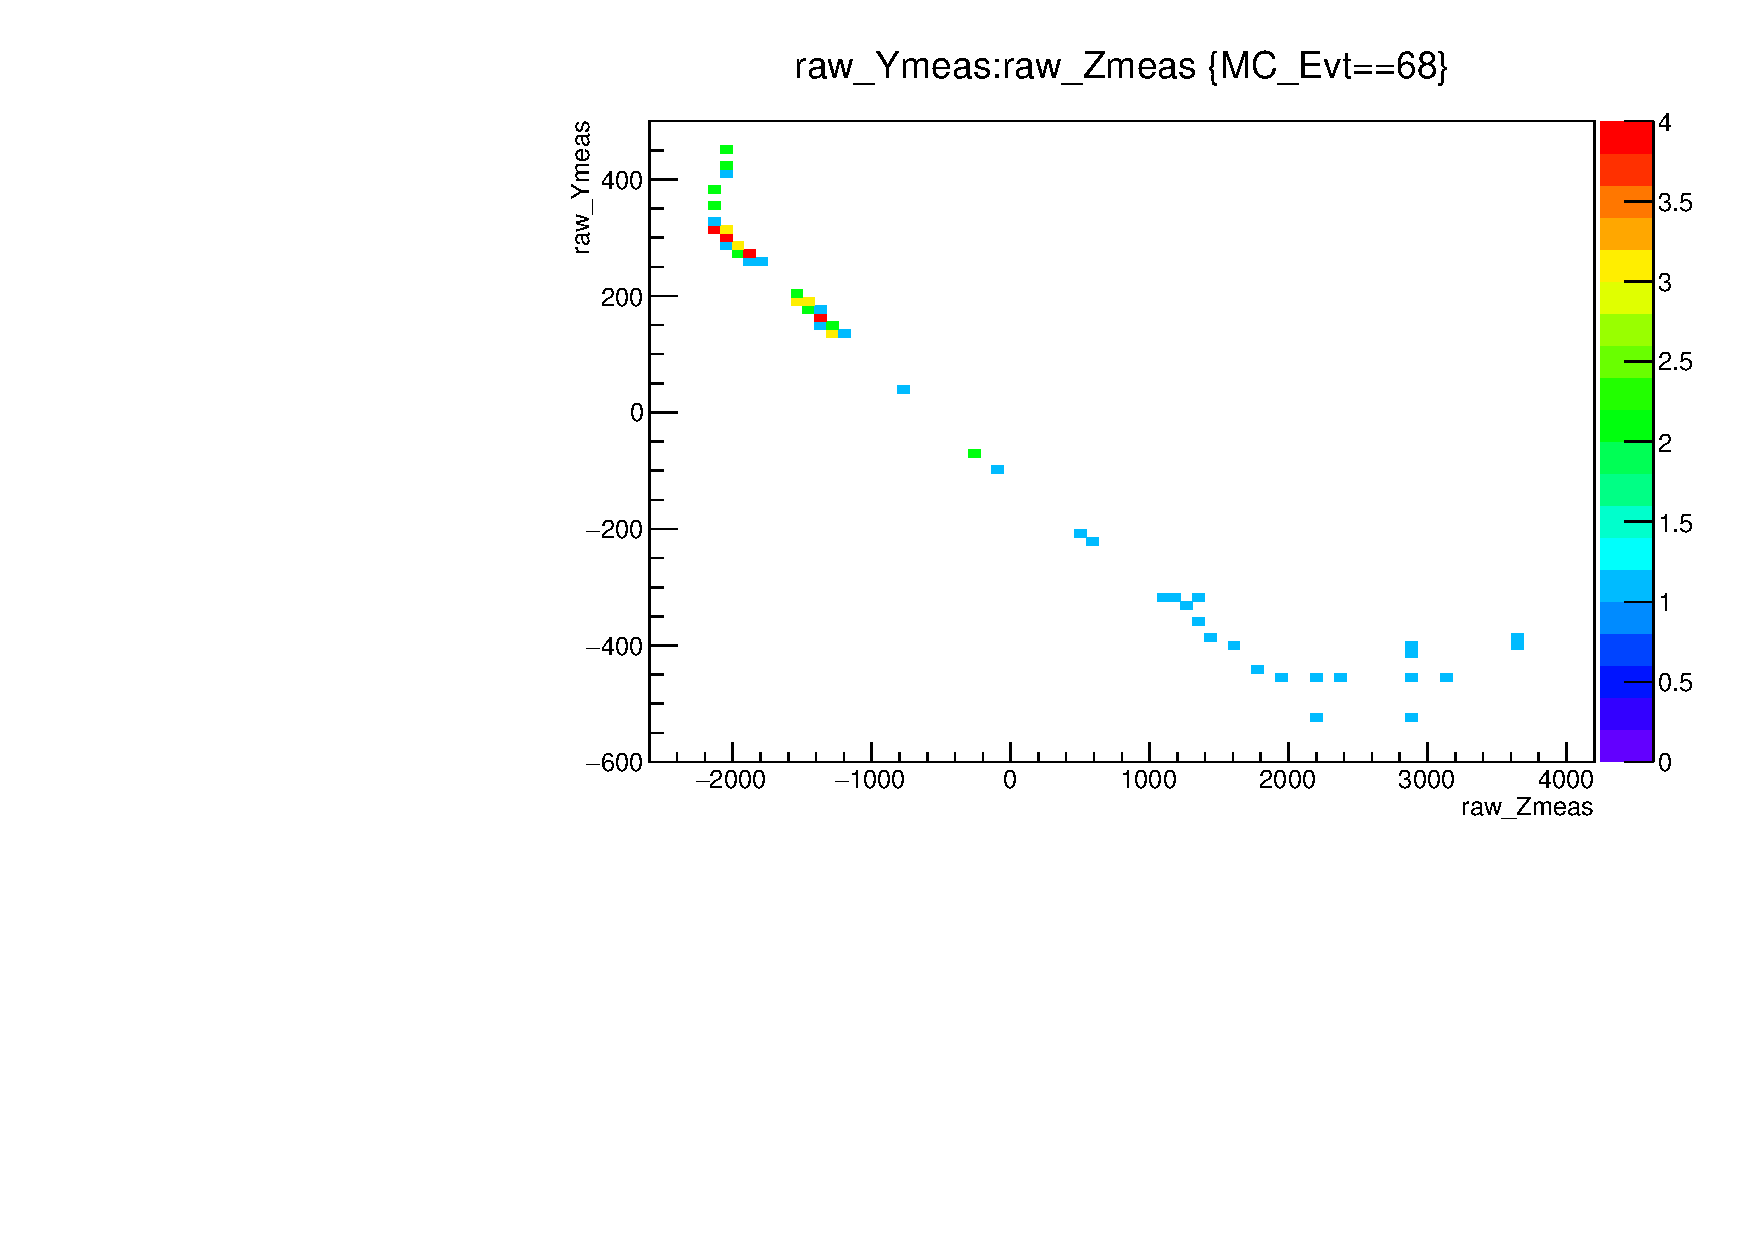
\includegraphics[width=0.9\textwidth]{figures/muCCQEorigin.pdf}}
		\caption[]{Example of a $\mu^{-}$ CCQE event which interacts in the TASD shown in in Y-Z profile. }
		%	\caption[]{Charge identification efficiency: out of reconstructed trajectories, how many are identified with the correct charge?
		\label{fig:event}
	\end{minipage}
\end{figure}


\begin{figure}[h!]
	\begin{minipage}{0.49\linewidth}
		\centerline{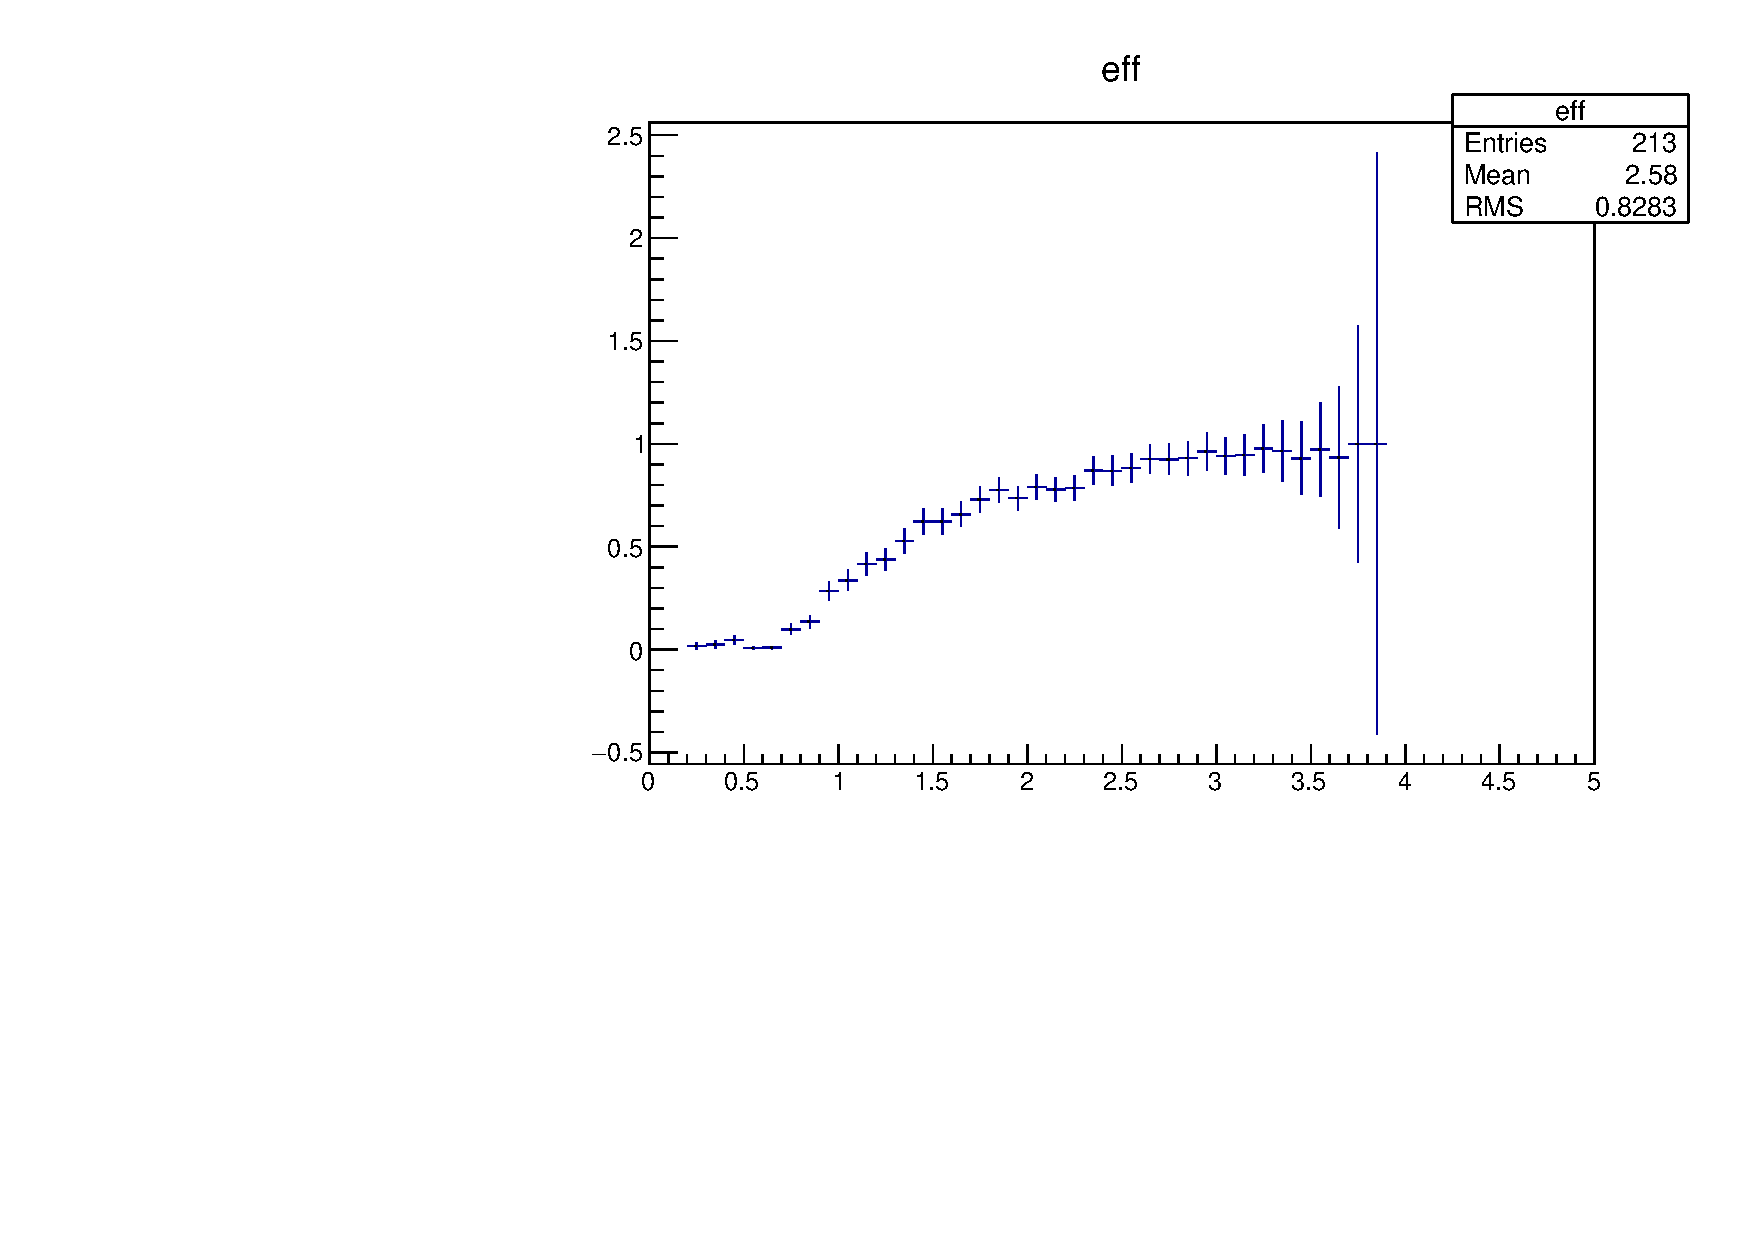
\includegraphics[width=0.9\linewidth]{figures/muNeutrinoFitted.pdf}}
		%\caption[]{ Reconstruction efficiency: out of identified trajectories, how many are reconstructed?}
			\caption[]{Reconstruction efficiency for a single $\nu_{\mu}$ beam}
		\label{fig:numufitted}
	\end{minipage}
	\hfill
	\begin{minipage}{0.49\linewidth}
		\centerline{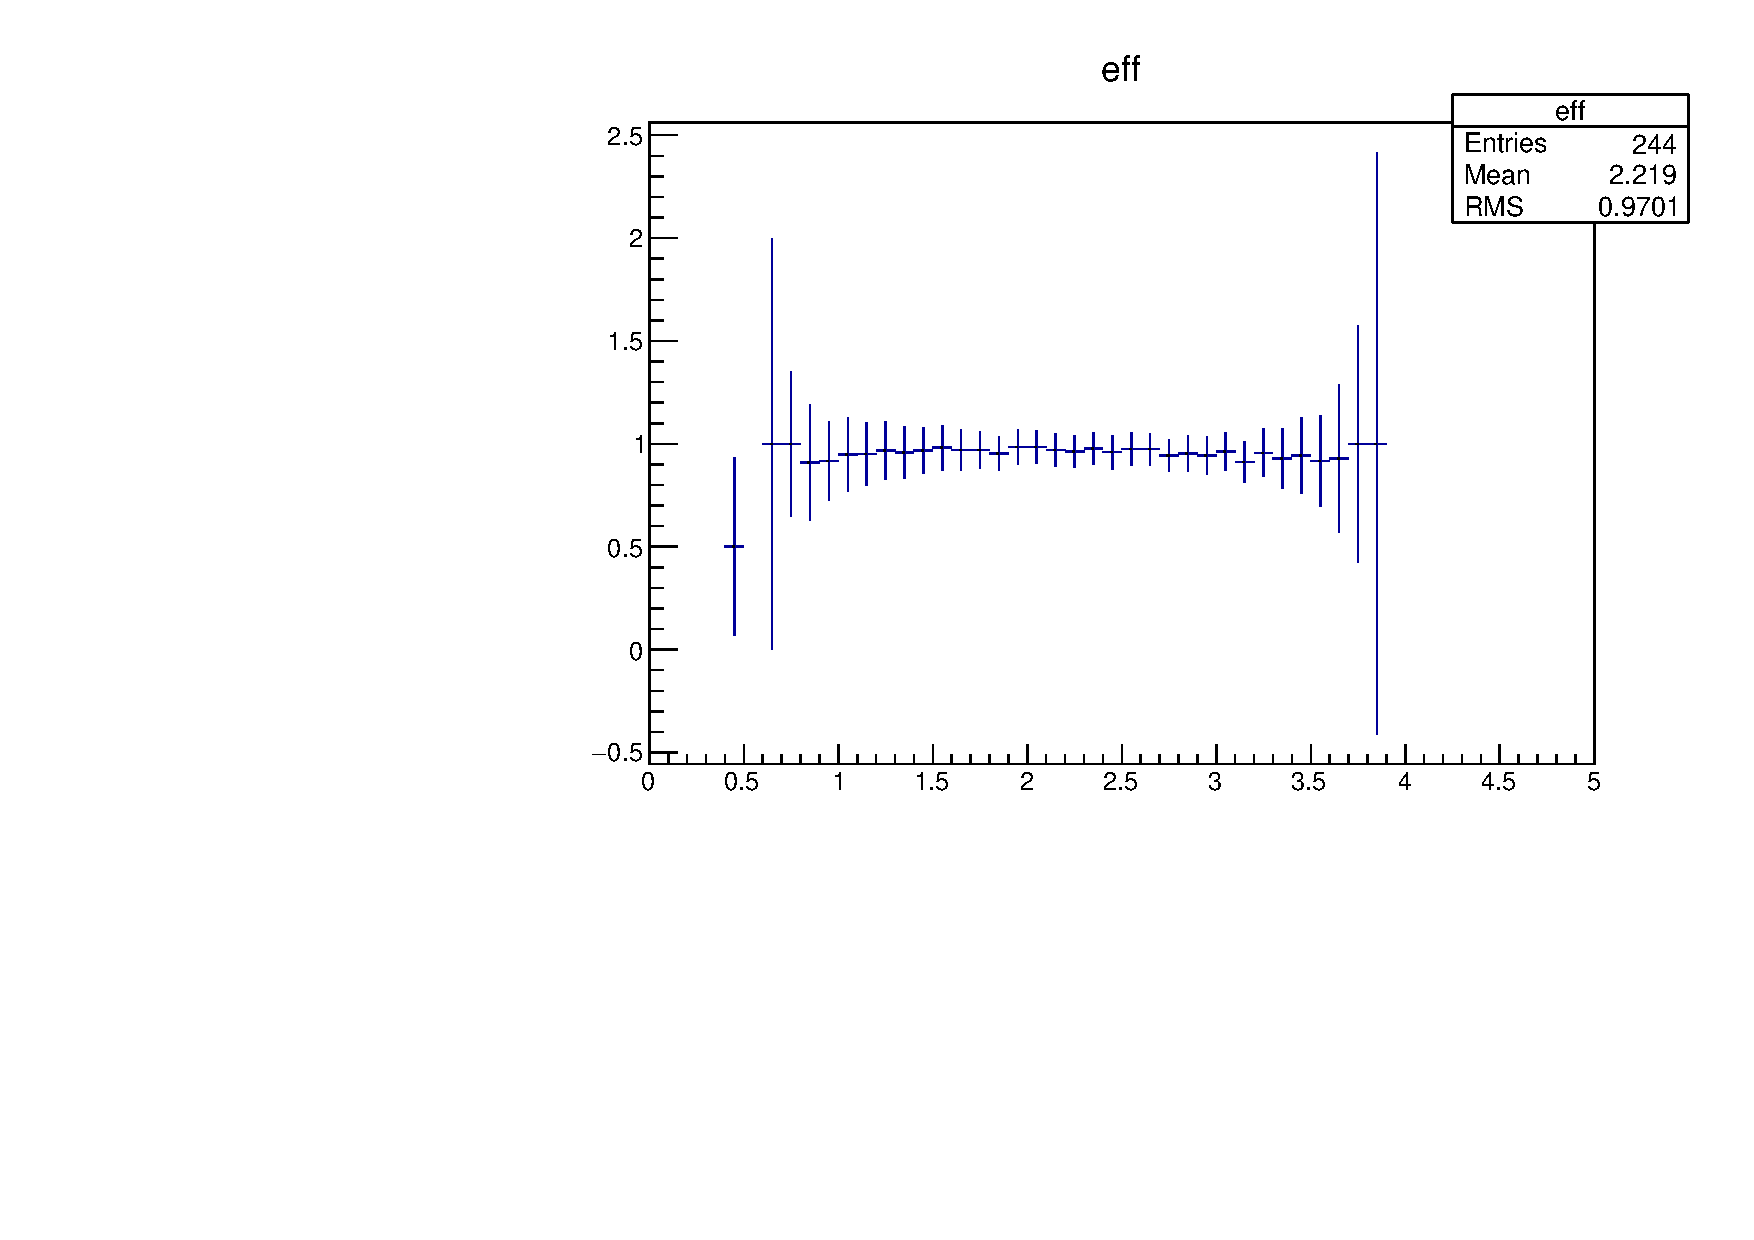
\includegraphics[width=0.9\textwidth]{figures/muNeutrinochargeID.pdf}}
		\caption[]{Charge identification efficiency for a single  $\nu_{\mu}$ beam}
		%	\caption[]{Charge identification efficiency: out of reconstructed trajectories, how many are identified with the correct charge?
		\label{fig:numucharge}
	\end{minipage}
\end{figure}

\begin{figure}[h!]
	\begin{minipage}{0.49\linewidth}
		\centerline{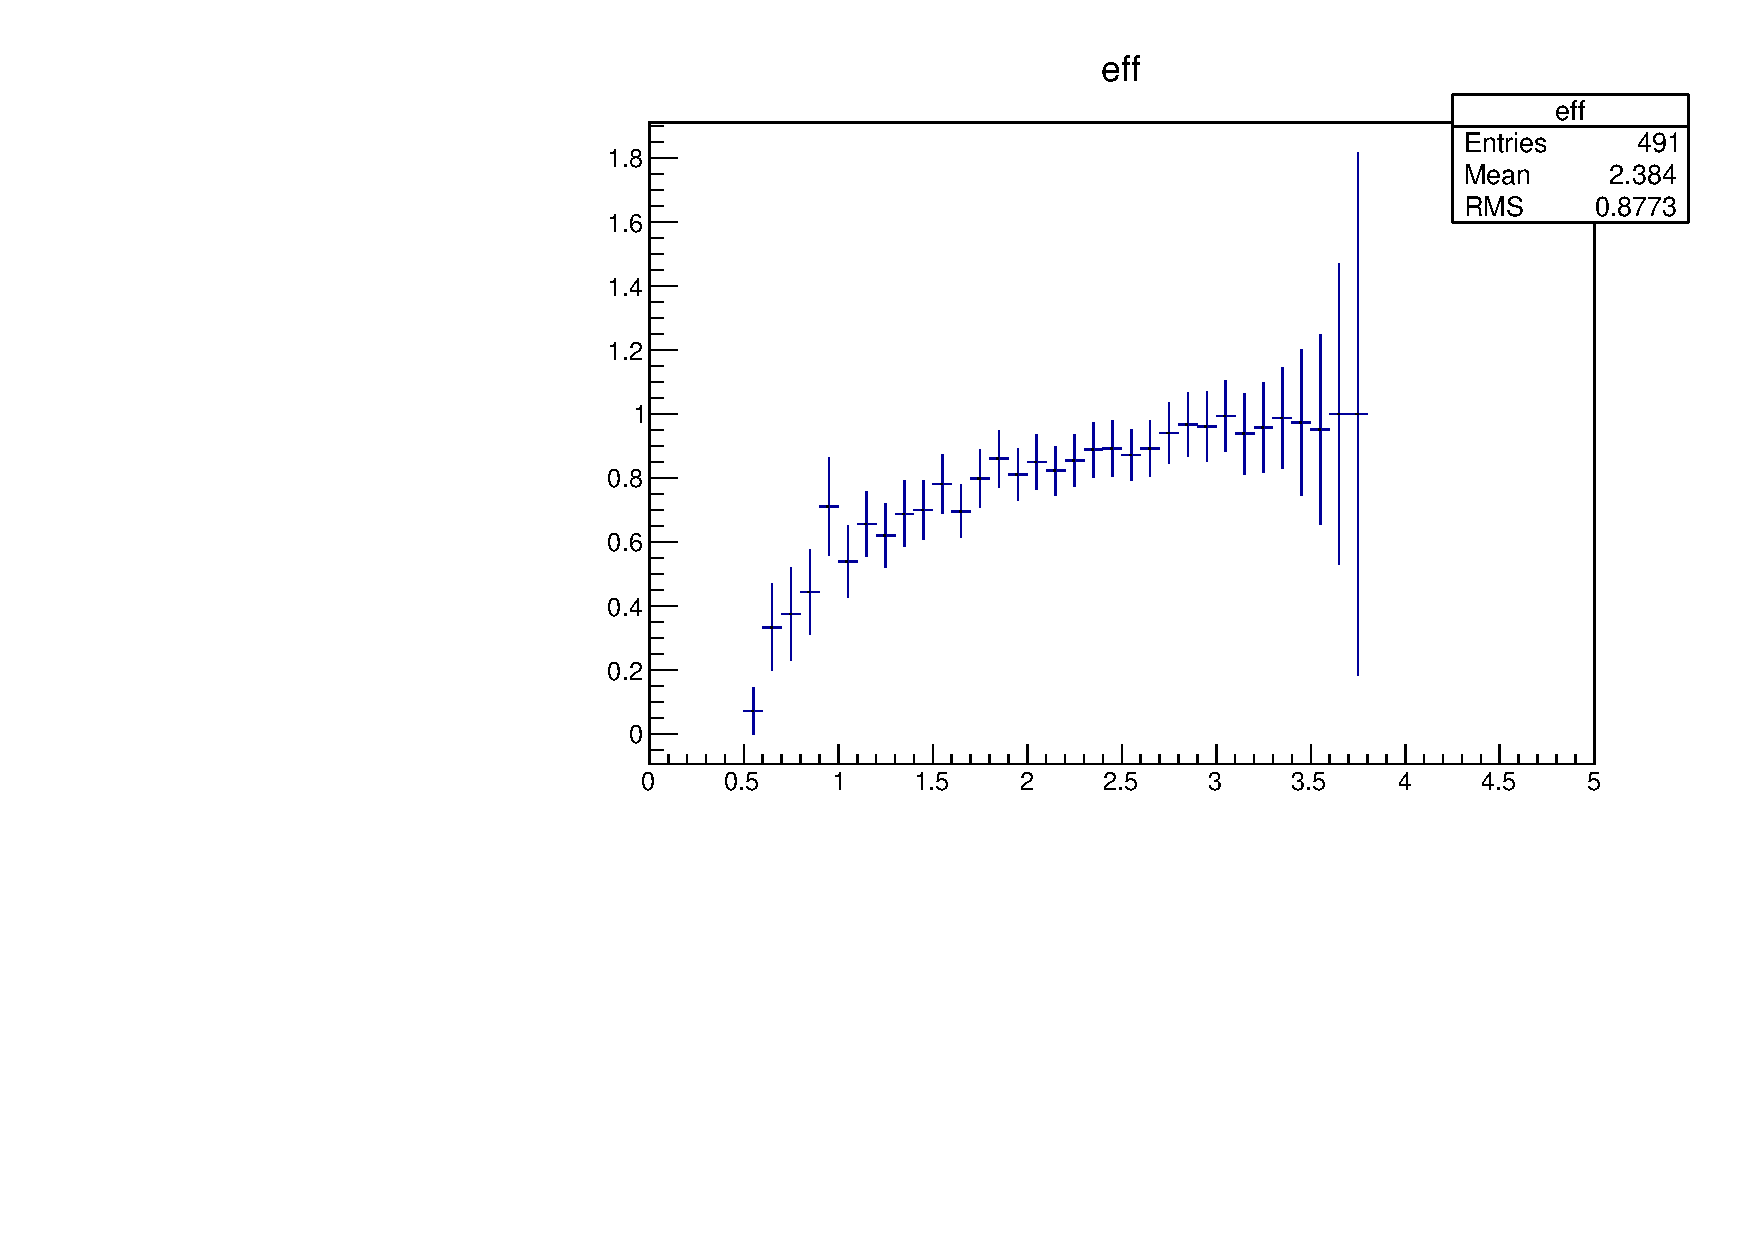
\includegraphics[width=0.9\linewidth]{figures/antimuNeutrinoFitted.pdf}}
		%\caption[]{ Reconstruction efficiency: out of identified trajectories, how many are reconstructed?}
			\caption[]{Reconstruction efficiency for a single $\bar{\nu_{\mu}}$ beam}
		\label{fig:antinumufitted}
	\end{minipage}
	\hfill
	\begin{minipage}{0.49\linewidth}
		\centerline{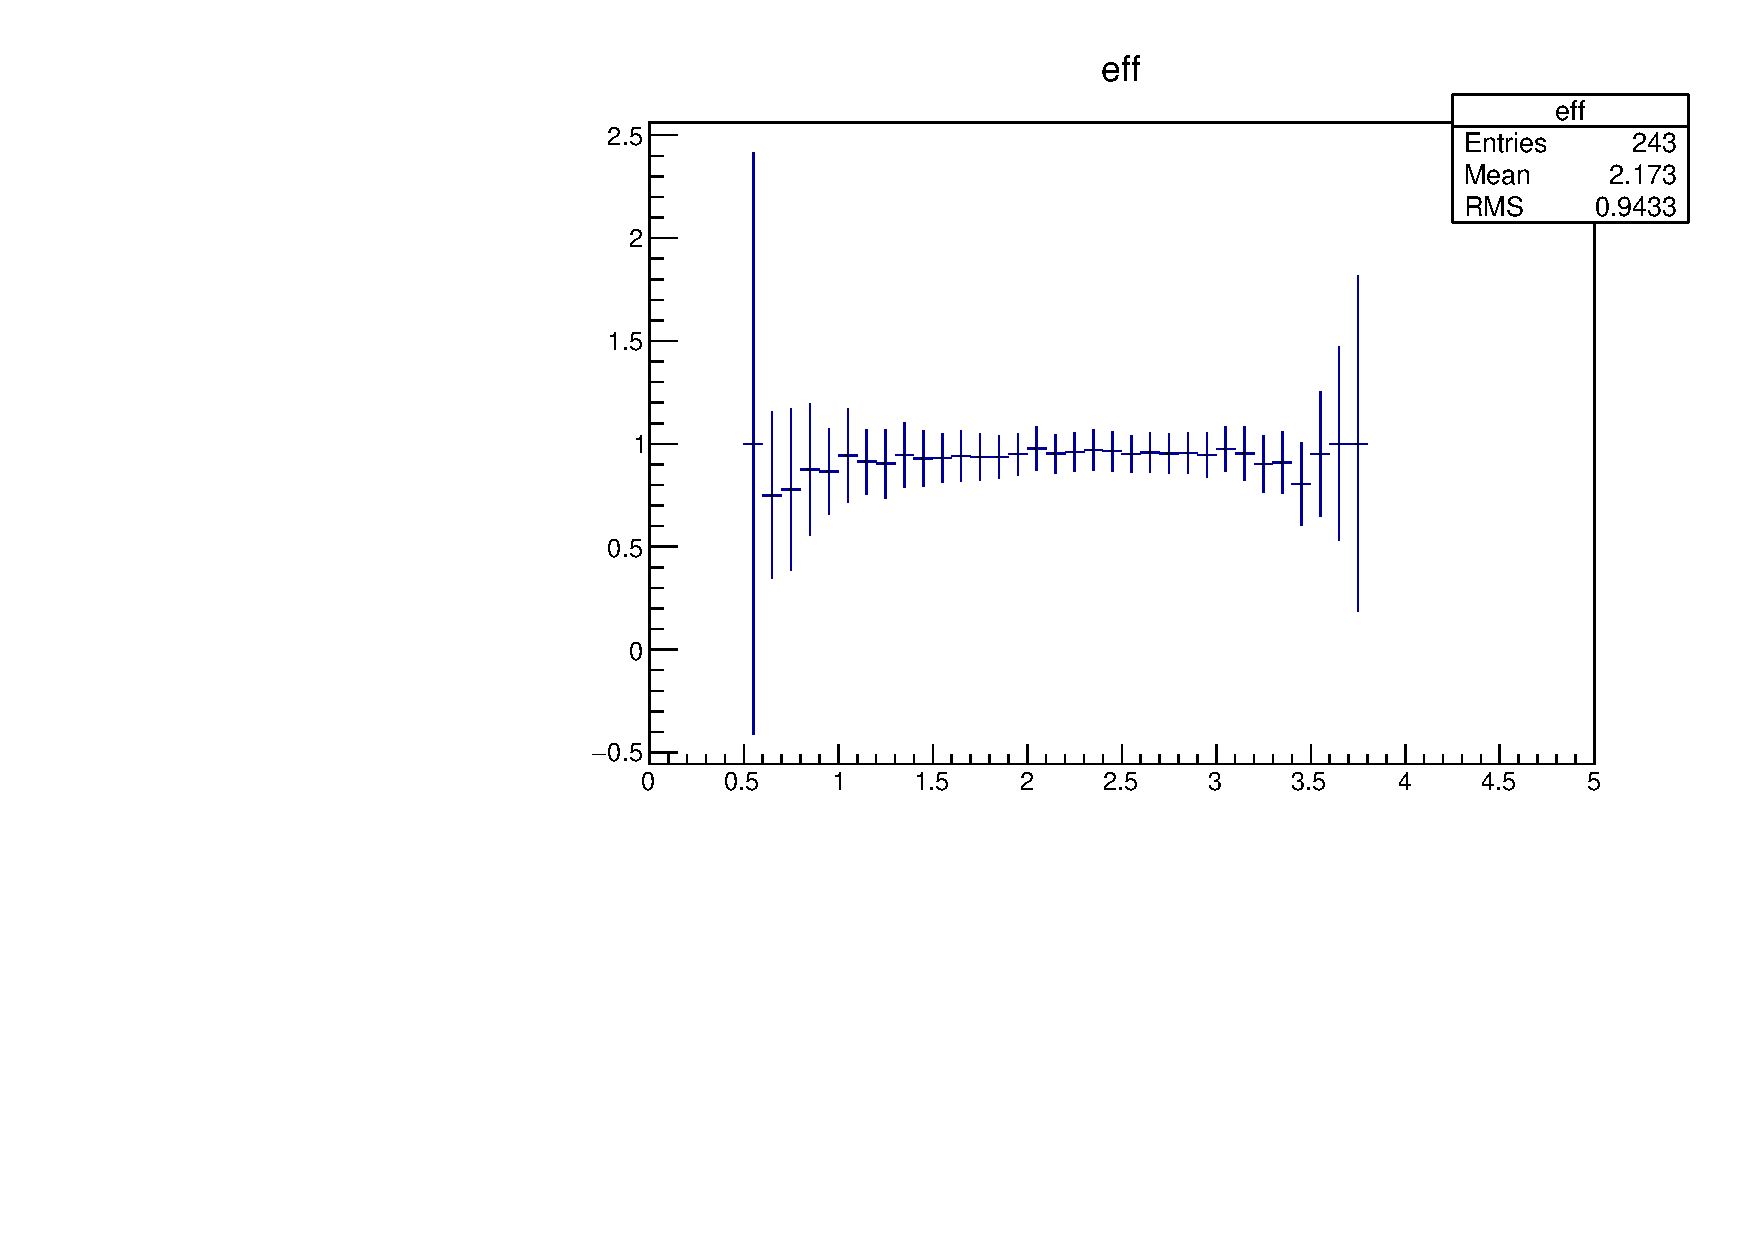
\includegraphics[width=0.9\textwidth]{figures/antimuNeutrinochargeID.pdf}}
		\caption[]{Charge identification efficiency for a single $\bar{\nu_{\mu}}$ beam}
		%	\caption[]{Charge identification efficiency: out of reconstructed trajectories, how many are identified with the correct charge?
		\label{fig:antinumucharge}
	\end{minipage}
\end{figure}

\begin{figure}[h!]
	\begin{minipage}{0.49\linewidth}
		\centerline{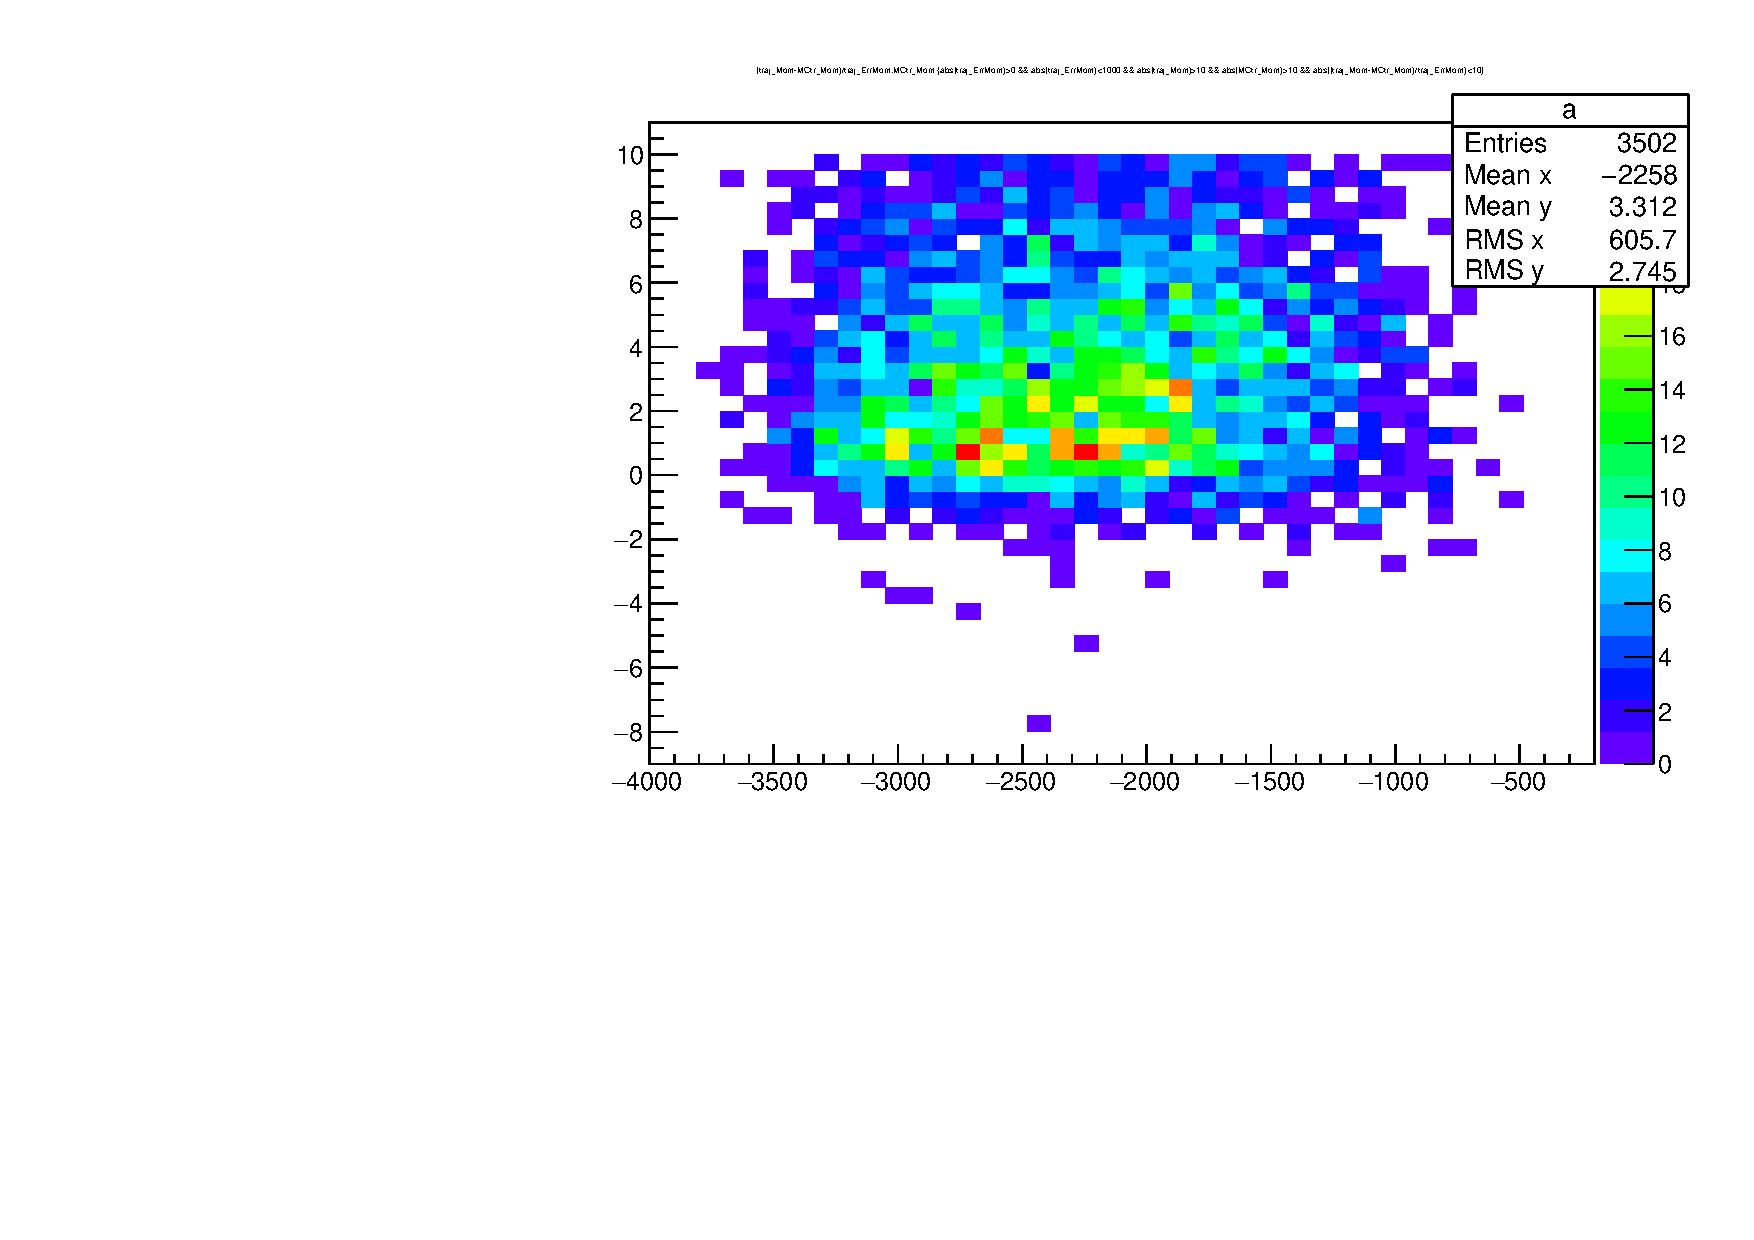
\includegraphics[width=0.9\linewidth]{figures/muNeutrinoPull.pdf}}
		%\caption[]{ Reconstruction efficiency: out of identified trajectories, how many are reconstructed?}
			\caption[]{Momentum pull plot for a single $\nu_{\mu}$ beam}
		\label{fig:numumom}
	\end{minipage}
	\hfill
	\begin{minipage}{0.49\linewidth}
		\centerline{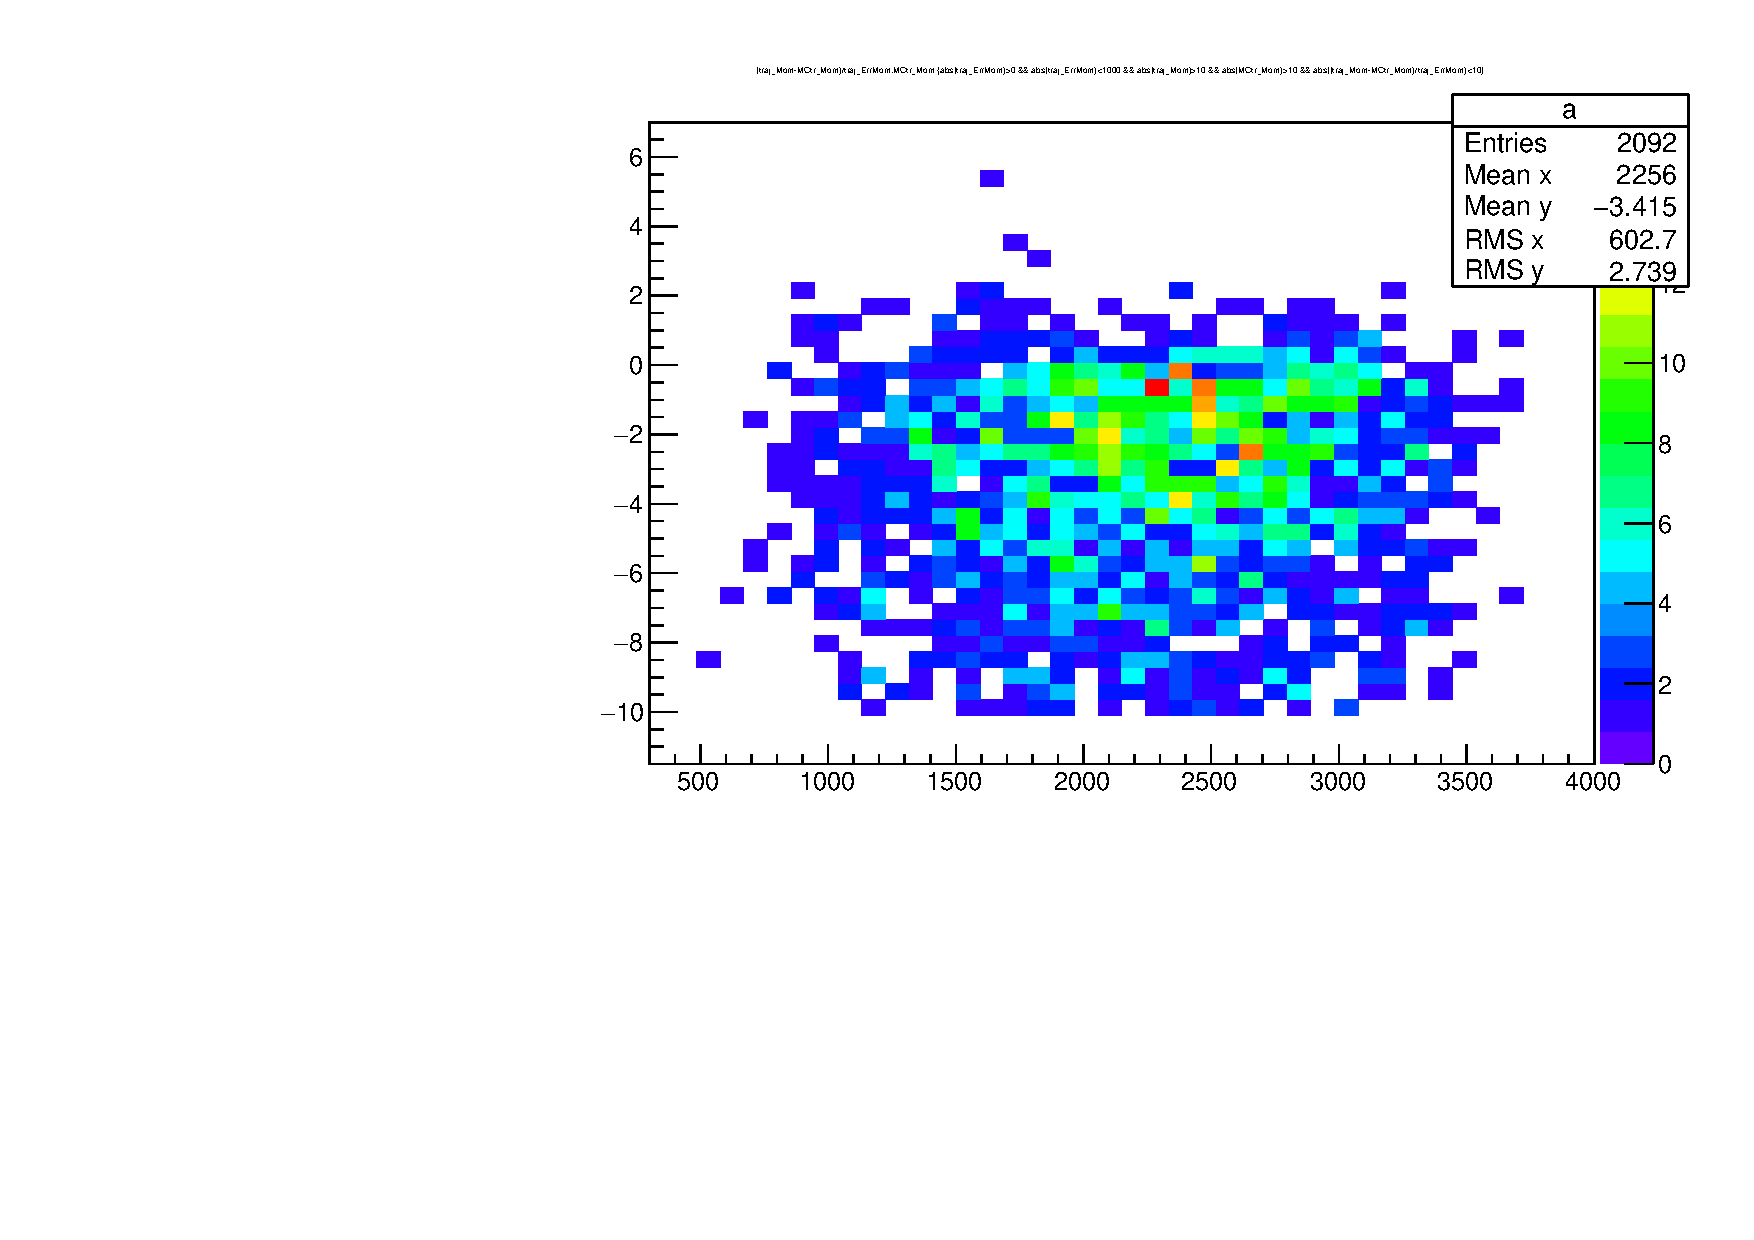
\includegraphics[width=0.9\textwidth]{figures/antimuNeutrinoPull.pdf}}
		\caption[]{Momentum pull plot for a single $\bar{\nu_{\mu}}$ beam}
		%	\caption[]{Charge identification efficiency: out of reconstructed trajectories, how many are identified with the correct charge?
		\label{fig:antinumumom}
	\end{minipage}
\end{figure}


\chapter{Presented last year}

\section{Presented as Future work last year}
\subsection{Software}
The largest task is to improve the reconstruction algorithms to better classify the events and identify both the momentum and charge. 
Current results seem to show that the main issue is to choose the optimum hits when there is multiple occupancy.

This was improved and corrected in time for the testbeam performed in June of last year.

\subsection{Hardware}
The electronics has been developed at the University of Geneva and will be tested at two test beams in June and July 2016. The current plan is to travel to CERN in June to perform tests with the electronics, to characterise the electronics in the laboratory and in the test beam and to emulate it in the digitization software.

This was tested and the digitization software confirmed with the acquisition of testbeam data.

\subsection{Physics performance}
The main goal is to establish the performance of a MIND type detector in terms of position, angle, momentum and energy resolution and to characterise the particle identification and charge separation. 
Another goal is to benchmark MIND simulations and reconstruction algorithms and compare them with experimental results.

From previous MIND type detectors studies carried out in the context of the Neutrino Factory~\cite{25NUfact}, charge current interactions are of the most interest for a MIND detector since they leave a clearer muon track. Reconstructions of electron tracks become more complex due to much shorter tracks and their similarity to hadronic showers. More detailed tests of electron beams will lead to further understanding of such events.

This is still ongoing. Neutrino tracks can be reconstructed in SaRoMaN, however many bugs have been discovered and have taken more time than expected.

\subsection{Neutrino interaction physics}
The ultimate goal of the research is to characterise neutrino interactions in the WAGASCI detector, identified using Baby MIND to determine the expected cross-section ratio between CC events in water and in carbon. 

This was not achieved and is still seen as a goal to be achieved in August when the detector will be shipped to Japan.

\section{Outline for the "last" 12 months}
\subsection{Software objectives}
\begin{itemize}
\item Launch a complete version of the SaRoMaN software package by June 2016.
\item Integrate the SaRoMaN and WAGASCI software packages by September 2016.
\end{itemize}
\subsection{Physics objectives}
\begin{itemize}
\item Perform physics studies of non-standard neutrino interactions (NSI) by October 2016.
\item Analysis of test beam at CERN by October 2016.
\item Perform neutrino cross-section studies with WAGASCI by February 2017.
\item Perform full Baby MIND beam tests characterization by June 2017.
\end{itemize}
\subsection{Hardware objectives}
\begin{itemize}
\item Perform electronics Front End Board beam test at CERN by July 2016.
\item Finalize Baby MIND by February 2017.
\end{itemize}

Most of these goals were achieved. SaRoMaN has been launched as a complete version and was launched on time. Unfortunately the WAGASCI collaboration has not shared their software so no integration has been made. NSI studies have not been conducted since unfortunately the collaboration with Durham has not been worked at. The electronics test beam and test beam analysis were performed on time. The full Baby MIND will be characterised this June and the design was finalised now in April 2017. Unfortunately neutrino cross-section studies with WAGASCI has not been started since the design has not been fully shared. However they were stated in January with another target design. Several bugs were discovered during these studies, this combined with time spend on other hardware related studies meant that the studies have not yet been completed but they will be completed by September 2017.

\chapter{Outline for the next 12 months}
\section{Objectives}
\label{a:objectives}
\subsection{Software objectives}
\begin{itemize}
\item Improve the SaRoMaN package reconstruction for Neutrino events by September 2017.
\end{itemize}
\subsection{Physics objectives}
\begin{itemize}
\item Perform physics studies of non-standard neutrino interactions (NSI) by October 2017.
\item Analysis of second test beam at CERN by October 2017.
\item Perform neutrino cross-section studies with WAGASCI by December 2017.
\item Perform neutrino cross-section studies with data from WAGASCI by March 2018.
\end{itemize}

\section{Future work}
\subsection{Physics performance}
The main goal is to establish the performance of a MIND type detector in terms of position, angle, momentum and energy resolution and to characterise the particle identification and charge separation. 
Another goal is to benchmark MIND simulations and reconstruction algorithms and compare them with experimental results.

From previous MIND type detectors studies carried out in the context of the Neutrino Factory~\cite{25NUfact}, charge current interactions are of the most interest for a MIND detector since they leave a clearer muon track.

This is still ongoing. Neutrino tracks can be reconstructed in SaRoMaN, however many bugs have been discovered and have taken more time than expected.

\subsection{Neutrino interaction physics}
The ultimate goal of the research is to characterise neutrino interactions in the WAGASCI detector, identified using Baby MIND to determine the expected cross-section ratio between CC events in water and in carbon. 


\section{Gantt chart}

Figure~\ref{fig:Gantt} shows a combined chart of the timeline for Baby MIND and for what conferences I will be aiming for and where I will be. Combined with the objectives given in section~\ref{a:objectives} provides a good plan and outline for the next 6 months.

\begin{figure}[h!]
\centering
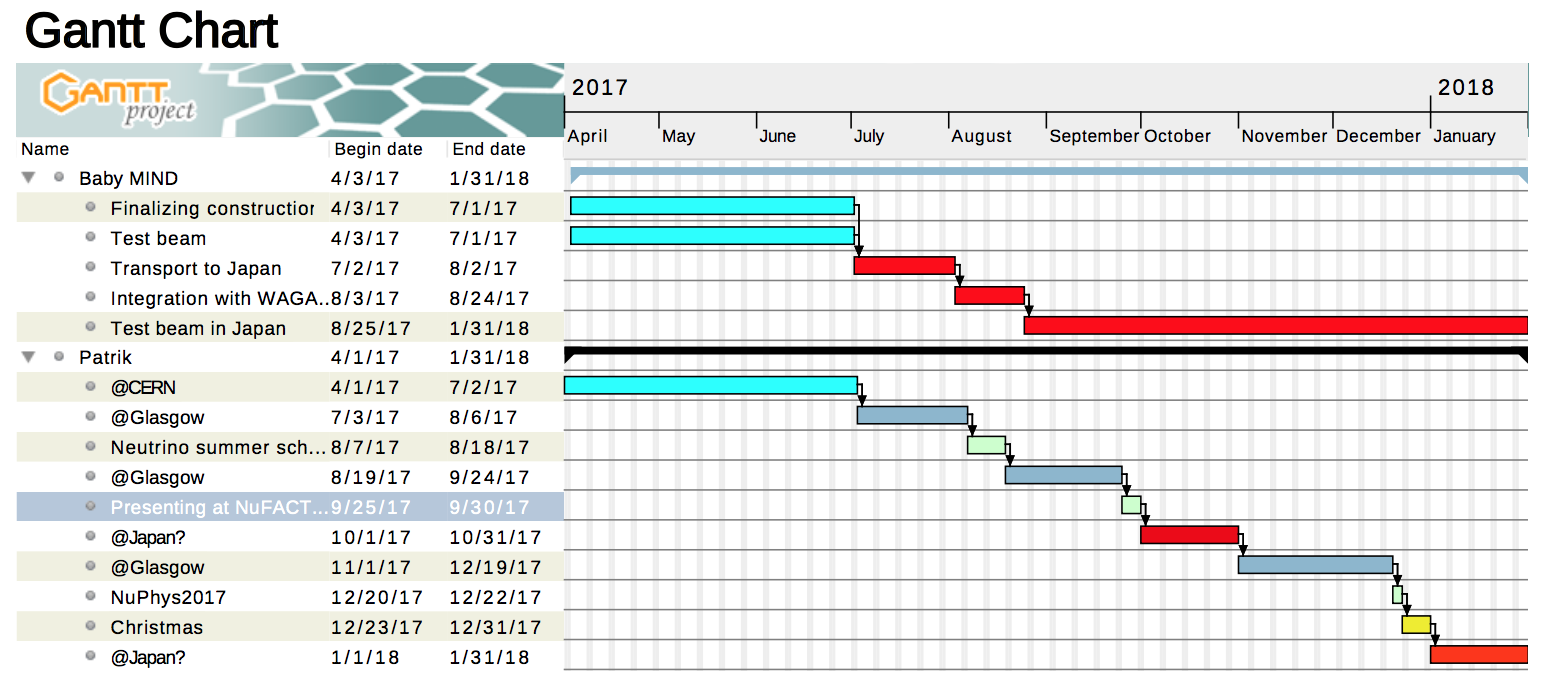
\includegraphics[width=\textwidth]{figures/Gantt.png}
\caption{A Gantt chart for the next 12 months.}
\label{fig:Gantt}
\end{figure}



%INCLUDE NEW Gantt chart.
%\begin{figure}[h!]
%\centering
%\includegraphics[width=\textwidth]{ghant.pdf}
%\caption{A Gantt chart for the next 12 months.}
%\label{fig:Gantt}
%\end{figure}

